%-------------------------------------------------------------------------------
%                      Template Naskah Skripsi
%               	Berdasarkan format JTETI FT UGM
% 						(c) @gunturdputra 2014
%-------------------------------------------------------------------------------

%Template pembuatan naskah skripsi.
\documentclass{jtetiskripsi}

%Untuk prefiks pada daftar gambar dan tabel
\usepackage[titles]{tocloft}
\renewcommand\cftfigpresnum{Gambar\  }
\renewcommand\cfttabpresnum{Tabel\   }

%Untuk hyperlink dan table of content
\usepackage[hidelinks]{hyperref}
\newlength{\mylenf}
\settowidth{\mylenf}{\cftfigpresnum}
\setlength{\cftfignumwidth}{\dimexpr\mylenf+2em}
\setlength{\cfttabnumwidth}{\dimexpr\mylenf+2em}

%Untuk Bold Face pada Keterangan Gambar
\usepackage[labelfont=bf]{caption}

%Untuk caption dan subcaption
\usepackage{caption}
\usepackage{subcaption}

%pdf
\usepackage{pdfpages}

%table
% \usepackage{longtable}
\usepackage{graphics}

\usepackage{wrapfig}


%equation
\usepackage{amsmath}

%hypenat
%\usepackage[none]{hyphenat}/

%bibliography
\usepackage{natbib}

%-----------------------------------------------------------------
%Disini awal masukan untuk data proposal skripsi
%-----------------------------------------------------------------
\titleind{Deteksi Keliling Luka menggunakan \break \emph{Active Contour (Snakes)} dan \emph{Gradient Vector Flow} (GVF) }

\fullname{Muhamad Rizki}

\idnum{3145160661}

%\approvaldate{-}
\approvaldate{-}

\degree{Sarjana Ilmu Komputer}

\yearsubmit{2020}

\program{Ilmu Komputer}

\dept{Ilmu Komputer}

% \firstsupervisor{Med Irzal, M. Kom.}
% \firstnip{197706152003121001}

\firstsupervisor{Muhammad Eka Suryana, M. Kom.}
\firstnip{198512232012121002}

\secondsupervisor{-}
\secondnip{-}

%hypenation


%-----------------------------------------------------------------
%Disini akhir masukan untuk data proposal skripsi
%-----------------------------------------------------------------

\tolerance=1
\emergencystretch=\maxdimen
\hyphenpenalty=10000
\hbadness=10000

\begin{document}
\cover
%-----------------------------------------------------------------

%-----------------------------------------------------------------
%Disini akhir masukan untuk muka skripsi
%-----------------------------------------------------------------

\tableofcontents 
\addcontentsline{toc}{chapter}{DAFTAR ISI}
\listoffigures
\addcontentsline{toc}{chapter}{DAFTAR GAMBAR}
\listoftables
\addcontentsline{toc}{chapter}{DAFTAR TABEL}

\begin{counterpage}
\end{counterpage}
%Disini awal masukan untuk Bab
%-----------------------------------------------------------------
%!TEX root = ./template-skripsi.tex
%-------------------------------------------------------------------------------
% 								BAB I
% 							LATAR BELAKANG
%-------------------------------------------------------------------------------

\chapter{PENDAHULUAN}
\section{Latar Belakang Masalah}

Salah satu organ yang sangat penting pada tubuh manusia adalah kulit. Ketika kulit terluka, diperlukan perawatan luka yang baik agar tidak terjadi infeksi. Luka adalah keadaan di mana fungsi anatomis kulit normal mengalami kerusakan akibat proses patologis yang berasal dari internal maupun eksternal dan mengenai organ tertentu. Proses penyembuhan luka terjadi melalui beberapa fase, yaitu: hemostasis (beberapa jam pasca-terjadinya luka), inflamasi (1 – 3 hari), proliferasi (4 – 21 hari), dan \emph{remodelling} (21 hari – 1 tahun). Fase-fase penyembuhan luka terjadi secara bertahap, namun dapat terjadi secara bersamaan (\emph{overlap}) \citep{pat2018:1}. %fine

Luka kronis adalah kondisi di mana luka mengalami proses penyembuhan yang tidak normal dengan durasi fase-fase yang sesuai \citep{landen2016transition:2}, kondisi ini dapat berkaitan dengan berbagai faktor yang memperlambat penyembuhan luka seperti adanya penyakit kronis, insufisiensi vaskuler, diabetes, gangguan nutrisi, penuaan, dan berbagai faktor lokal pada luka (tekanan, infeksi, dan edema). Secara umum, luka kronis dapat terjadi akibat ulkus vena, ulkus arteri, ulkus dekubitus, dan ulkus diabetik \citep{zhao2016inflammation:3}. %fine

Setiap tahunnya prevalensi luka secara umum mengalami peningkatan. 1.4 juta orang dewasa dirawat karena luka kekerasan di tahun 2000 sampai 2010, 1,6\% di antaranya dirawat di Unit Gawat Darurat (UGD) di Amerika Serikat \citep{monuteaux2017cross:4}. Berdasarkan hasil Riset kesehatan dasar (Riskesdas) tahun 2018, prevalensi luka di Indonesia selalu mengalami peningkatan dari tahun 2007 sebanyak 7,5\%, tahun 2013 sebanyak 8,2\%, dan di tahun 2018 sebanyak 9.2\% \citep{hasilkesehatan2018riset}. %fine

Luka kronis bisa jadi merupakan komplikasi pada penderita Diabetes Melitus (DM). Sebanyak 15\% dari seluruh populasi penderita DM memiliki komplikasi berupa luka diabetes \citep{fard2007assessment:6}. Prevalensi Diabetes Melitus di Indonesia kategori penduduk umur 15 tahun keatas pada tahun 2018 adalah 2\% \citep{hasilkesehatan2018riset}. Pada tahun 2030 diprediksi meningkat menjadi 21,3 juta orang. Indonesia menempati peringkat keempat jumlah penderita DM terbanyak di dunia \citep{wild2004global:7}. %fine

Berdasarkan hasil prevalensi, luka kronis menjadi permasalahan bagi perawat luka dan instansi kesehatan terkait. Selain itu diperlukan penanganan khusus dalam proses pemulihan luka kronis. Permasalahan luka kronis menghadirkan kesulitan berat bagi yang menderita kondisi ini dan beban keuangan untuk industri kesehatan. Di sisi klien dapat berdampak pada penurunan kualitas hidup, ketidakmampuan untuk melakukan fungsi tubuh secara optimal, serta tingginya kebutuhan finansial. Bahkan dalam beberapa kasus dapat menyebabkan amputasi dan kematian. Bagi instansi kesehatan terkait akan memberikan dampak pada tingginya pembayaran asuransi kesehatan dikarenakan frekuensi perawatan luka yang dilakukan paling tidak 2,4 kali per minggu di mana menghabiskan 66\% waktu perawat luka \citep{HSE2007:8}. Di Amerika Serikat , luka kronis setiap tahunnya menelan biaya \$20 miliar dan memengaruhi 5,7 juta orang \citep{brown2018wearable:9}. Berdasarkan data dari alodokter.com, biaya perawatan luka di Indonesia berkisar mulai dari antara Rp61.500,00–Rp267.000,00 belum termasuk biaya balutan. %fine

Salah satu tanggung jawab perawat luka profesional adalah melakukan pengkajian pada luka, di mana hasil pengkajian tersebut bermanfaat untuk menentukan pemberian balutan luka yang tepat, memonitor perbaikan luka dan mencegah komplikasi sehingga perawatan akan menjadi \emph{cost effective} \citep{benbow2016best:10}. %fine

% jelaskan pentingnya deteksi tepi pada pengkajian luka (bab 1).
Salah satu hal yang mendasar dalam proses penyembuhan luka kronis adalah melihat ukuran luka, dan umumnya hal ini adalah kriteria pertama yang harus dipertimbangkan dalam proses \emph{assessment} luka yang mana hal ini memiliki peran penting di antaranya memantau laju dan kemajuan penyembuhan, mengevaluasi efektivitas perawatan, dan mengidentifikasi luka. Selain itu perubahan ukuran luka memungkinkan kita dalam mengamati tingkat penutupan, waktu penutupan, pelebaran, dan wawasan lain yang merupakan indikator untuk memprediksi status penyembuhan \citep{carrion2022automatic}. Masih digunakannya metode konvensional seperti mengukur menggunakan penggaris memiliki tingkat akurasi dan reliabilitas rendah sehingga perawat terkesan lambat dalam memberikan perawatan dibandingkan dengan profesi kesehatan yang lain seperti dokter. Sebuah studi menyatakan standar teknik pengukuran perawatan yang melibatkan penggunaan perkiraan penggaris dan mata telanjang, memiliki tingkat kesalahan 44\% \citep{budman2015design:11}. Untuk mengatasi ketidakakuratan pengukuran manual, maka metode pengukuran keliling luka berbasis analisa citra (\emph{image}), khususnya citra biomedis (\emph{biomedical image}) dan citra medis (\emph{medical image}) perlu dikembangkan. %fine

Saat ini penelitian \emph{state of the art} telah dilakukan untuk analisis luka. Banyak studi yang menjelaskan evaluasi luka menggunakan citra luka untuk mengetahui status luka. Citra medis dapat mengirimkan informasi lebih banyak untuk para ahli kesehatan daripada deskripsi subjektif yang cenderung menimbulkan kesalahan interpretasi. Lebih jauh lagi, gambar citra luka dapat digunakan untuk mentransmisi informasi tentang status penyembuhan untuk konsultasi medis di lokasi pedalaman. Pada sebuah percobaan tahun 2013, ditemukan nilai tinggi yang dihubungkan ke galeri foto luka di aplikasi mobile dan pelacakan luka melalui progresi grafis. Sehingga, untuk meningkatkan fitur citra diperlukan pengembangan algoritma analisis citra untuk penentuan ukuran dan warna dari foto luka yang diambil dari kamera telepon pintar atau kamera tablet \citep{poon2015algorithms:12}. %fine

Ketika sebuah foto diambil dengan pose yang sama oleh kamera yang berbeda, warna yang tersimpan mungkin berbeda, ini merupakan salah satu penelitian paling awal untuk analisis luka. Salah satu solusi untuk masalah tersebut adalah menggunakan format \emph{device independent} sRGB. Semua vendor kamera setidaknya menawarkan mode ini tetapi default ke format RGB mereka sendiri. Menggunakan \emph{chart} referensi warna ketika gambar citra luka diambil, Poucke et. al., berhasil melakukan mekanisme kalibrasi antara perangkat \emph{device dependent} RGB ke sRGB dengan mentransformasi citra terlebih dahulu menjadi ruang warna CIE \emph{colorimetric}, kemudian ke sRGB melalui serangkaian masalah optimisasi \citep{van2010automatic:13}. %fine

Upaya untuk menentukan batas luka oleh kamera telah dilaporkan dalam beberapa penelitian. Wang et. al. mengembangkan kotak pengambilan gambar dengan kamera \emph{smartphone} \& dua cermin, untuk menangkap gambar ulkus kaki dasar. Batas selanjutnya disempurnakan dengan algoritma \emph{mean-shift} kemudian disetel lagi dengan \emph{Region Adjacency Graph}. Setelah batas diperoleh, K-means dijalankan untuk mengukur rasio warna RYB. Metode ini dievaluasi pada 34 pasien yang berbeda di klinik Worcester. Kemudian penelitian Wang, masih berkonsentrasi pada penentuan batas luka tetapi dengan SVM \citep{wang2016area:15}. Pelabelan manual kumpulan data 100 luka yang menghasilkan 10.000 wilayah dilakukan oleh tim dokter (tiga ekspert) di sekolah kedokteran UMASS. Metode kerjanya sebagai berikut, pertama citra disegmentasi menjadi superpiksel dengan SLIC. Kemudian deskriptor warna \& tekstur diekstraksi untuk persiapan setiap tahap SVM. Pada tahap pertama, warna \& Tas kata diekstraksi dengan DSIFT. Selama tahap kedua, warna \& tekstur \emph{wavelet} diekstraksi. Tahap SVM pertama menjalankan k-binary SVM \emph{classifier} dilatih pada set citra yang berbeda. Pada tahap kedua, set kesalahan klasifikasi dilatih lagi dengan SVM biner. Setelah selesai, hasilnya sekali lagi disempurnakan dengan \emph{Conditional Random Field}. Meskipun memberikan hasil yang memuaskan, semua percobaan diuji pada ulkus kaki (\emph{close wound}) \citep{wang2014smartphone:14}. %fine

Friesen dari University of Manitoba memimpin tim peneliti untuk melakukan serangkaian penelitian dalam analisis luka. White et. al., sebagai tim peneliti pertama yang berkonsentrasi untuk mengukur ukuran luka ulkus tekan dilakukan dalam tiga langkah. Pertama, mengukur jarak dari kamera ke luka dengan referensi fokus. Kedua, kalibrasi pose kamera dari penggabungan data sensor (akselerometer, magnetometer \& giroskop). Ketiga, Jepit \& perbesar untuk mengukur ukuran luka dari referensi yang sebelumnya diketahui \citep{white2014algorithms:16}. Sayangnya, penyimpangan (\emph{drift}) dari ukuran sebenarnya di atas cukup besar karena setiap langkah meningkatkan \emph{drift}. Poon et. al., Yang melanjutkan penelitian mempertahankan fokus yang sama, kecuali jarak luka. Metode batas luka telah diubah menjadi \emph{Grabcut}, maka setiap citra yang diambil diproyeksikan ke bidang 2d untuk menstabilkan sudut. Akhirnya warna tersegmentasi menjadi warna RYB \citep{poon2015algorithms:17}. Salah satu kelemahan dari pendekatan yang diambil, deteksi batas dengan \emph{Grabcut} hanya dapat dijalankan secara semi-otomatis, karena membutuhkan penyesuaian parameter. %fine

Setelah batas luka telah ditentukan dengan benar, dapat digunakan untuk memproduksi \emph{gel bioprinting} untuk penutupan luka. Gholami, \emph{et. al.}, mengevaluasi tujuh algoritma untuk memenuhi tujuan ini \citep{gholami2017segmentation:18}. Tiga algoritma yang dibandingkan adalah dari berbasis tepi, tiga lainnya berdasarkan pertumbuhan wilayah, dan satu lainnya berdasarkan tekstur. Algoritma \emph{Livewire} yang didasarkan pada tepi adalah yang terbaik di antaranya. Berdasarkan kajian teori di atas, \emph{grabcut} digunakan sebagai segmentasi wilayah luka dan warna citra luka dikonversi menjadi \emph{Commission internationale de l'éclairage} (CIE) untuk membuat mekanisme kalibrasi. %fine

Salah satu metode yang banyak digunakan dalam aplikasi pemrosesan citra medis dan biomedis adalah metode kontur aktif (\emph{active contour}) atau yang lebih dikenal dengan sebutan \emph{snake} yang diperkenalkan oleh M. Kass et. al. pada tahun 1988 \citep{kass1988snakes:21}. Sebuah \emph{active contour} (\emph{snake}) adalah kurva yang meminimalkan fungsi energi untuk kondisi tertentu. Fungsi energi ini biasanya terdiri dari dua istilah: energi internal, yang membatasi kelancaran (\emph{smoothness}) dan kekencangan (\emph{tautness}) kontur, dan energi eksternal, yang menarik kontur elastis ke fitur-fitur menarik \citep{acton2007biomedical:19}. Penelitian ini berfokus pada implementasi metode \emph{snake} dalam mendeteksi keliling luka kronis. %fine
% !
%Karena potensi \emph{active contour} yang diusulkan M. Kass et al. tahun 1988, banyak model dari modifikasi \emph{snake} tradisional(dasar), salah satunya adalah \emph{Gradient vector flow} (GVF) yang diusulkan Xu et. al. pada tahun 1998.
% !
Ada kesulitan pada metode \emph{snake} tradisional. Pertama kontur awal yang harus dekat dengan target, dengan kata lain jangkauan tangkap (\emph{capture range}) \emph{snake} terbatas. Masalah kedua ialah \emph{snake} tradisional tidak dapat mengerakkan kontur ke dalam cekungan batas (\emph{concave boundary}) \citep{guo2013review:20} \citep{xu1998snakes:22}. 

%Masalah \emph{capture range} dan \emph{concave boundary} sepenuhnya berhasil diatasi oleh \emph{Gradient vector flow} (GVF) \emph{snake} yang diusulkan oleh Xu dan Prince \citep{xu1998snakes:22}\citep{acton2007biomedical:19}. Dengan menggunakan beberapa contoh dua dimensi dan satu contoh tiga dimensi, menunjukkan bahwa GVF memiliki jangkauan tangkapan besar dan mampu memindahkan ular ke batas cekung\citep{xu1998snakes:22}.
% !
%Meskipun masalah terkait dengan \emph{active contour} sebagian besar telah diatasi oleh Xu et. al. yaitu dengan GVF, akan tetapi metode GVF memiliki kelemahan karena terkadang hasil dari kontur berhenti di tepi palsu (\emph{spurious edges})\citep{abdullah2016robust}. 
%(copy)
%Abdullah, et. al. dalam penelitian tentang segmentasi iris berhasil mengatasi kelemahan dari metode GVF dengan metode yang mereka usulkan, yaitu menambahkan \emph{pressure force} pada GVF. Arah pergerakan \emph{active contour} disesuaikan dengan kelopak mata sehingga menghasilkan hasil yang akurat dan efisien\citep{abdullah2016robust}.
Abdullah, et. al. dalam penelitian tentang segmentasi iris berhasil mengatasi kelemahan dari metode \emph{snake} dengan metode yang mereka usulkan, yaitu menambahkan \emph{pressure force} pada \emph{snake}. Arah pergerakan \emph{snake} disesuaikan dengan kelopak mata sehingga menghasilkan hasil yang akurat dan efisien \citep{abdullah2016robust}.

Penulis tertarik menerapkan metode \emph{snake} pada penelitian ini dengan alasan metode ini adalah metode yang umum digunakan dalam aplikasi pemrosesan citra medis dan biomedis. Selain itu, \emph{snake} cocok untuk mendeteksi objek dengan bentuk bebas \emph{(free-form object)} seperti halnya dengan citra luka kronis. Dikutip dari jurnal \emph{Medical and Biological Image Analysis} tahun 2018, \emph{snake} telah banyak dan baik digunakan dalam berbagai aplikasi seperti segmentasi CT-Scan otak, segmentasi untuk deteksi kanker payudara, deteksi lesi (bintik) pada kulit dan lain-lain \citep{hemalatha2018active}. %fine
% !
Secara ideal, penulis ingin juga menerapkan metode yang dikembangkan oleh \citep{abdullah2016robust}, namun hal tersebut belum dapat dilakukan karena harus memahami lebih terlebih dahulu tentang \emph{snake}, maka dari itu untuk penelitian ini dibatasi menggunakan metode \emph{active contour} saja. Penelitian ini akan berfokus pada pengembangan metode \emph{snake} dalam mendeteksi keliling luka kronis.

\emph{Dataset} citra yang penulis gunakan untuk penelitian ini didapat dari penelitian luka \mbox{Ns. Ratna Aryani, M.Kep}, tahun 2018 \mbox{\citep{ratna2018rancang}} yang tersedia di \emph{repository} \url{https://github.com/mekas/InjuryDetection}. Penelitian ini dilakukan sampai mendapatkan hasil berupa nilai akurasi yang didapat dari selisih area kurva akhir \emph{snake} terhadap luas area \emph{ground truth} (nilai sebenarnya).



\section{Rumusan Masalah}
Berdasarkan Latar belakang yang telah dikemukakan di atas. Fokus permasalahan pada penelitian ini adalah “Bagaimana cara mendeteksi keliling luka kronis menggunakan metode \emph{Active contour} (\emph{Snake}) dan \emph{active contour} yang ditambahkan interpolasi ?”.

\section{Pembatasan Masalah}
\begin{enumerate}
	\item Pendeteksian keliling luka kronis menggunakan \emph{snake} dan \emph{snake} yang ditambahkan interpolasi menggunakan data citra luka yang didapat dari penelitian luka \mbox{Ns. Ratna Aryani, M.Kep}, tahun 2018 \mbox{\citep{ratna2018rancang}}.
	\item Penelitian dilakukan sampai mendapatkan hasil, yaitu nilai akurasi dari selisih area kurva \emph{snake} terhadap area \emph{ground truth}
\end{enumerate}

\section{Tujuan Penelitian}
Tujuan penelitian ini adalah untuk mengetahui hasil dari metode \emph{snake} dan \emph{snake} yang ditambahkan interpolasi dalam mendeteksi keliling luka kronis.

\section{Manfaat Penelitian}
\begin{enumerate}
	\item Bagi peneliti
		
	Penelitian ini merupakan media penerapan ilmu pengetahuan, khususnya dalam pengembangan metode \emph{Active contour} pada pengkajian luka kronis.
		
	\item Instansi terkait 
	 	
	 	Metode yang diajukan diharapkan dapat membuka peluang untuk diajukan ke instansi kesehatan terkait dalam proses pengkajian luka kronis.	
	 	
	 \item Bagi ilmu pengetahuan
	 	\begin{itemize}
	 		\item Mahasiswa
	 			
	 			Diharapkan penelitian ini dapat digunakan sebagai penunjang referensi, khususnya pustaka tentang deteksi keliling menggunakan \emph{Active contour}.
	 			
	 		\item Bagi peneliti selanjutnya
	 			
	 			Diharapkan Penelitian ini dapat digunakan sebgai dasar atau kajian awal bagi peneliti lain yang ingin meneliti permasalahan yang sama.
	 			
	 	\end{itemize}	
\end{enumerate}


% Baris ini digunakan untuk membantu dalam melakukan sitasi
% Karena diapit dengan comment, maka baris ini akan diabaikan
% oleh compiler LaTeX.
\begin{comment}
\bibliography{daftar-pustaka}
\end{comment}

%!TEX root = ./template-skripsi.tex
%-------------------------------------------------------------------------------
%                            BAB II
%               KAJIAN TEORI
%-------------------------------------------------------------------------------

\chapter{KAJIAN PUSTAKA}                


\section{Populasi dan Sampel}
Tujuan dari sebuah riset adalah untuk memperoleh informasi dari populasi. Populasi merupakan seluruh kumpulan elemen yang dapat digunakan untuk membuat kesimpulan tertentu sedangkan sampel merupakan kelompok yang dipilih dari populasi untuk digunakan dalam riset. Sampai saat ini belum ada kesepakatan atau ketentuan secara ideal dalam menentukan berapa banyak sampel dalam penelitian. Sampel yang baik adalah sampel yang mencerminkan populasinya \citep{amirullah2015metode}. Ukuran sampel harus diperhatikan dalam melakukan penelitian. Gay \& Diehl berpendapat bahwa ukuran sampel harus sebesar-besarnya, semakin besar ukuran sampel maka akan semakin representatif, ukuran sampel yang dapat diterima bergantung pada jenis penelitiannya sebagai berikut \citep{gay1992research}:
\begin{enumerate}
	\item Penelitian deskriptif sampel minimumnya 10\% dari populasi.
	\item Penelitian yang bersifat korelasional sampel minimunnya 30 subyek
	\item penelitian kausal-perbandingan, sampelnya sebanyak 30 subyek per grup
	\item penelitian eksperimental, sampel minimunnya adalah 15 subyek per grup.
\end{enumerate}
Fraenkel \& Wallen menyarankan besar minimum untuk ukuran sampel sebagai berikut \citep{fraenkel2012design}:
\begin{enumerate}
	\item Penelitian deskriptif sebanyak 100 sampel.
	\item Penelitian yang bersifat korelasional sebanyak 50.
	\item penelitian kausal-perbandingan sebanyak 30 per grup.
	\item penelitian eksperimental sebanyak adalah 30 atau 15.
\end{enumerate}

\section{Pengolahan Citra Digital (\emph{Digital Image Processing})}
Pengolahan citra digital adalah bidang ilmu yang mengacu pada pada pengolahan citra digital dengan menggunakan komputer digital. Citra digital terdiri dari sejumlah elemen yang masing-masing memiliki lokasi dan nilai tertentu. Elemen-elemen ini sering disebut dengan istilah piksel \citep{gonzalez2002digital}.
Citra dapat didefinisikan sebagai fungsi intensitas dua dimensi $I(x,y)$ yang direpresentasikan sebagai matriks berukuran $m$ x $n$ sebagai berikut:
\begin{figure}[H]
	\centering
	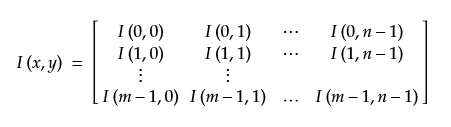
\includegraphics[width=0.8\textwidth]{gambar/image_intensity}
	\caption{Representasi Citra Digital}
	\label{Gambar:imageintensity}
\end{figure}
$m$ x $n$ menyatakan resolusi citra, dan setiap elemen dari matriks menyatakan sebuah piksel (\emph{picture element}). Nilai $I$ pada pasangan koordinat $(x,y)$ disebut intensitas (\emph{intensity}). Dalam operasi pengolahan citra, sebagian besar operasi dilakukan dalam citra \emph{grayscale} \citep{tyagi2018understanding}.

\subsection{Citra \emph{Grayscale}}
Citra \emph{grayscale} adalah citra yang hanya memiliki satu kanal (\emph{channel}) pada setiap pikselnya yang mewakili intensitas. Intensitas piksel berada dalam kisaran [0, 255] yang mana hal ini menunjukkan tingkat terangnya atau tingkat cahaya dari suatu pixel. Warna pada citra \emph{grayscale} merupakan warna abu dengan tingkatan dari hitam hingga sampai putih (tingkat keabuan). Kisaran intensitas piksel bernilai 0 artinya hitam dan 255 adalah putih (untuk \emph{256-graylevel}).
\begin{figure}[H]
	\centering
	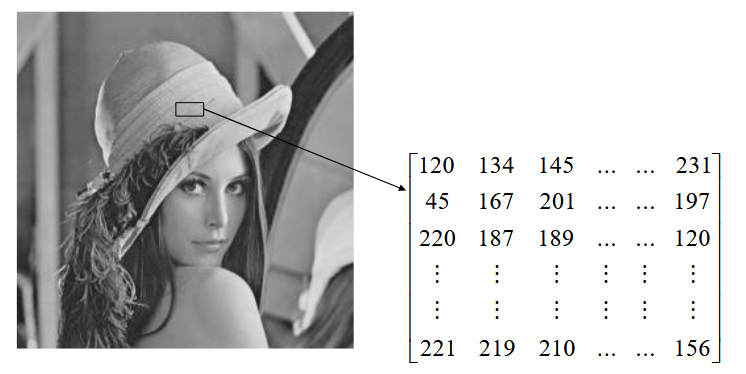
\includegraphics[width=0.5\textwidth]{gambar/grayimage}
	\caption{Contoh citra \emph{grayscale}}
	\label{Gambar:grayimage}
\end{figure}

Setiap piksel dalam citra umumnya dijelaksan oleh kombinasi tiga nilai intensitas R (\emph{red}), G (\emph{green}),dan B (\emph{blue}). Salah satu cara memetakan nilai tersebut ke satu nilai \emph{grayscale} adalah dengan menggunakan metode \emph{luminosity} \citep{kumar2016gray}.
\begin{equation}
	\label{luminosity}
	L(x,y) = 0.21 R (x,y) + 0.72 G (x,y) + 0.07 B (x,y).
\end{equation}
$L(x,y)$ melambangkan nilai intensitas \emph{grayscale} pada pasangan koordinat $(x, y)$. R, G, dan B masing-masing adalah nilai intensites citra \emph{channel} R (\emph{red}), G (\emph{green}),dan B (\emph{blue}) pada pasangan koordinat $(x,y)$

\begin{figure}[H]
	\centering
	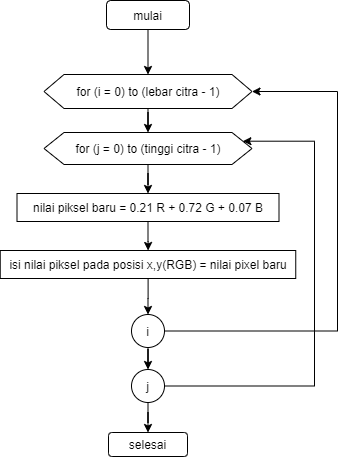
\includegraphics[width=0.45\textwidth]{diagram/grayscale}
	\caption{Proses konversi citra RGB menjadi \emph{grayscale}}
	\label{Gambar:grayscalediagram}
\end{figure}

\subsection{\emph{Gaussian Low Pass Filter} / \emph{Gaussian Filter}}
Peningkatan kualitas citra (\emph{image enhancement}) adalah proses mengedit citra untuk membuatnya 'lebih baik' untuk aplikasi tertentu \citep{tyagi2018understanding}. Hal ini melibatkan proses menghaluskan atau mempertajam konten citra. Salah satu metode dalam proses menghaluskan citra adalah \emph{filtering}, salah satunya adalah dengan menggunakan metode \emph{Gaussian filter}. Proses ini adalah proses memblur citra menggunakan fungsi Gaussian dengan tujuan mengurangi \emph{noise} citra dan mengurangi detail tertentu. Kernel gaussian \emph{Gaussian blur} $G(x,y)$ dideskripsikan sebagai berikut:
\begin{equation}
\label{gaussblur}
G(x,y) = {\frac{1}{2 \pi \sigma^2} e}^{-{\frac{x^2+y^2}{2 \sigma^2}}}
\end{equation}
$\sigma$ dan $e$ menujukkan standar deviasi dan konstanta logaritma natural ($e \approx 2,718281828459$), $x$ dan $y$ adalah posisi koordinat Kernel gaussian.



\section{Gradien citra (\emph{image gradient})}
Tepi (\emph{edge}) dalam ruang lingkup pengolahan citra digital mencirikan batas dari suatu objek dalam citra digital. Deteksi tepi (\emph{edge detection}) merupakan metode identifikasi objek dalam citra berbasis tepi. Salah satu metode deteksi tepi yang umum digunakan adalah metode gradien citra (\emph{image gradient}). Dalam konsep matematis, gradien dikenal sebagai turunan pertama (\emph{first-order derivatives}). Gradien dari citra $I$ dilambangkan dengan notasi $\nabla I$ dan di definisikan sebagai berikut:
\begin{equation}
	\label{gradientimagedefinition}
	{
		\nabla I =
	}
	{
		\begin{bmatrix}
			\nabla I (x,y)_x	\\
			\nabla I (x,y)_y
		\end{bmatrix}
	}
	{
		=
	}
	{
		\begin{bmatrix}
			\frac{\partial I (x,y)}{\partial x}	\\
			\frac{\partial I (x,y)}{\partial y}
		\end{bmatrix}
	}
\end{equation}
di mana $\nabla I (x,y)_x$ dan $\nabla I (x,y)_y$ masing-masing adalah persamaan gradien citra $I$ arah (\emph{direction}) $x$ dan $y$ yang dapat dihitung menggunakan dua persamaan berikut:
\begin{equation}
	\label{gradient_fd1}
	\nabla I (x,y)_x = I(x+1 , y) - I(x,y)
\end{equation}
\begin{equation}
	\label{gradient_fd2}
	\nabla I (x,y)_y = I(x , y + 1) - I(x,y)
\end{equation}
untuk besarnya (\emph{magnitude}) gradien $I$ dapat dihitung menggunakan persamaan berikut:
\begin{equation}
	\label{magnitudegradientfd}
	M(x,y) = ||\nabla I(x,y)|| = \sqrt{ (\nabla I (x,y)_x)^2 + (\nabla I (x,y)_y)^2 }
\end{equation}

Selain menggunakan persamaan (\ref{gradient_fd1}), (\ref{gradient_fd2}), dan (\ref{magnitudegradientfd}), perhitungan gradien citra dapat menggunakan operator gradien yang nantinya akan dikonvolusikan dengan citra. Salah satu operator gradien umum yang sering digunakan adalah operator Sobel/kernel Sobel. Konvolusi dilambangkan dengan $\ast$. Operator Sobel arah $x$ dan $y$, serta besar gradien Sobel masing-masing ditunjukkan oleh persamaan berikut:
\begin{equation}
	\label{sobel_x}
	G_x = 
	\begin{bmatrix}
		-1 & 0 & 1	\\
		-2 & 0 & 2	\\
		-1 & 0 & 1	
	\end{bmatrix}
\end{equation}
\begin{equation}
	\label{sobel_y}
	G_y = 
	\begin{bmatrix}
		1 & 2 & 1	\\
		0 & 0 & 0	\\
		-1 & -2 & -1	
	\end{bmatrix}
\end{equation}
\begin{equation}
	\label{sobel_mag}
	GS = | G_x \ast I(x,y) | + | G_y \ast I(x,y) |
\end{equation}

\begin{figure}[H]
	\centering
	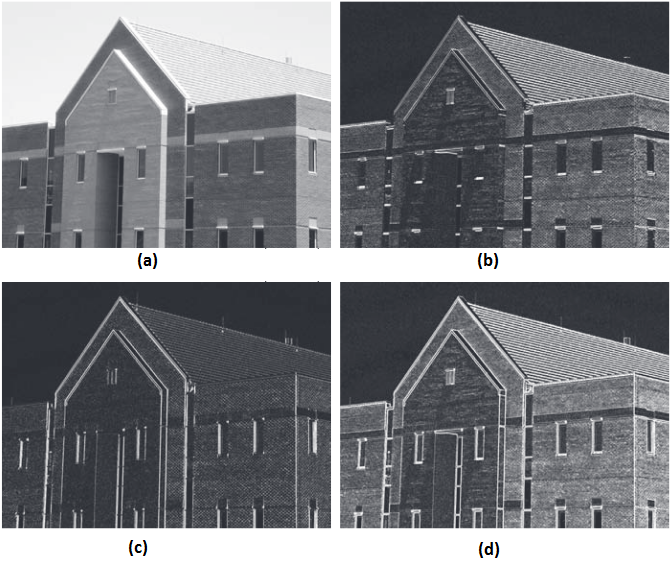
\includegraphics[width=0.8\textwidth]{gambar/sobel}
	\caption{(a) citra \emph{grayscale} ; (b) $|G_x \ast I(x,y)|$, gradien arah $x$ menggunakan kernel Sobel-x ; (c) $|G_y \ast I(x,y)|$, gradien arah $x$ menggunakan kernel Sobel-y ; (d) gradien citra, $| G_x \ast I(x,y) | + | G_y \ast I(x,y) |$ \citep{gonzalez2002digital}}
	\label{Gambar:sobel}
\end{figure}

\section{\emph{Active contour}}
\emph{Active contour} yang juga dikenal dengan sebutan \emph{snakes} adalah kurva yang di definisikan dalam citra (\emph{image}), kurva ini dapat bergerak menuju batas objek atau \emph{feature} dari sebuah citra yang dipengaruhi oleh dua fungsional energi yang disebut energi internal dan energi eksternal.
\begin{figure}[H]
	\centering
	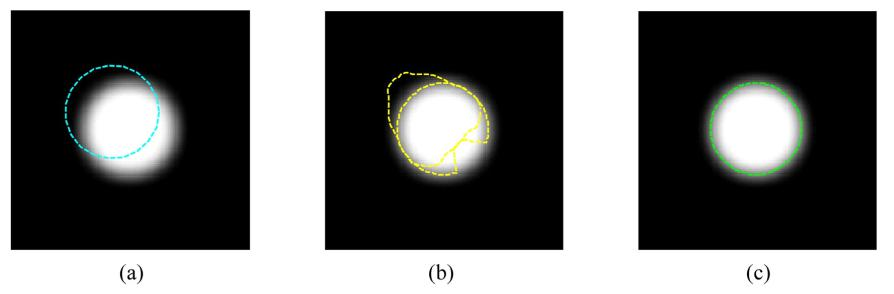
\includegraphics[width=1\textwidth]{gambar/snake1}
	\caption{(a) citra objek lingkaran \& \emph{initial snake}, (b) evolusi kurva \emph{snake},
		(c) bentuk akhir dari \emph{snake} setelah iterasi selesai \citep{acton2007biomedical:19}}
	\label{Gambar:snake1}
\end{figure}

\subsection{Representasi \emph{Snake}}
\emph{Snake} di representasikan sebagai kurva parametrik tertutup $\textbf{v}(s) = (x(s), y(s))$, di mana $s$ adalah panjang kurva dengan rentang tertentu, $x(s)$ dan $y(s)$ masing-masing merupakan elemen dari kurva $\textbf{v}$ pada saat $s$. Sebagai contoh diberikan sebuah kurva sebagai berikut:
\begin{figure}[H]
	\centering
	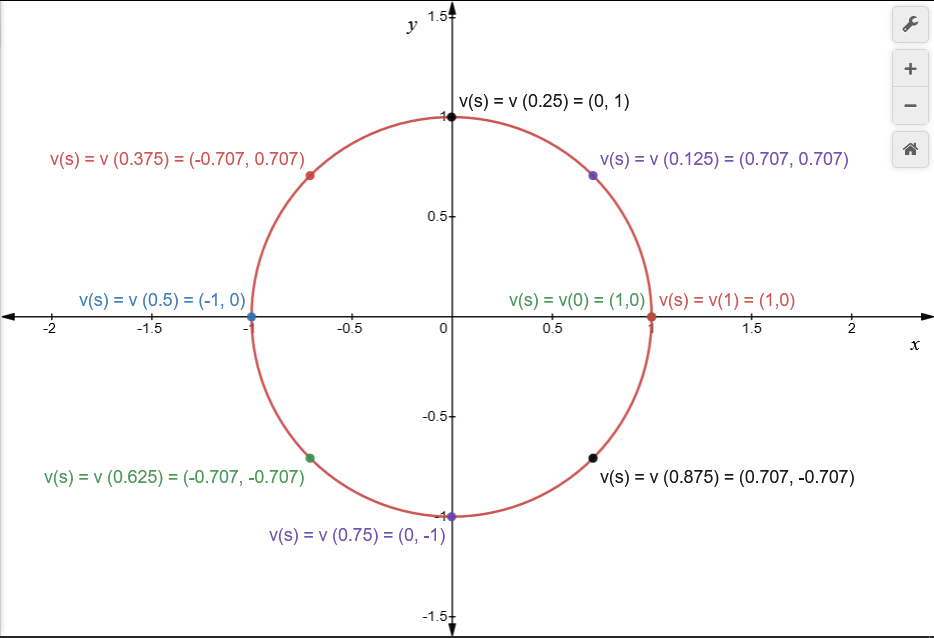
\includegraphics[width=1\textwidth]{gambar/k_lingkaran}
	\caption{Kurva ingkaran}
	\label{Gambar:k_lingkaran}
\end{figure}
Kurva di atas adalah kurva lingkaran $\textbf{v}(s) = [cos (2 \pi s), sin (2 \pi s)]$, $s \in [0, 1]$. Perlu diperhatikan bahwa titik awal $\textbf{v}(0)$ dan titik akhir $\textbf{v}(1)$ di definisikan sebagai titik yang sama.

Algoritma pembuatan lingkaran menggunakan bentuk parametrik (\emph{parametric form}) lingkaran adalah sebagai berikut:
\begin{figure}[H]
	\begin{lstlisting}[language=Python, basicstyle=\tiny]
		repeat until theta >= 360;
		{ 
			x = h + r*cos(theta)
			y = k + r*sin(theta)
			draw a line to x,y
			add step to theta
		}
	\end{lstlisting}
	\caption{\emph{source code} inisialisasi kurva lingkaran}
	\label{Gambar:algo_circle}
\end{figure}
yang dilakukan algoritma di atas adalah menghasilkan koordinat \texttt{x, y} dari sebuah titik pada lingkaran yang diberi sudut (\texttt{theta}). Dimulai dari \texttt{theta = 0} kemudian \emph{looping} sampai \texttt{theta = 360} atau \texttt{theta = $2\pi$}. \texttt{h} dan \texttt{k} adalah koordinat dari titik tengah lingkaran dan \texttt{r} adalah jari-jari lingkaran \citep{john_page}

Fungsional energi \emph{snake} di definisikan sebagai berikut \citep{abdullah2016robust}:
\begin{equation}
	\label{eq_1}
	E_{snake} = \int^1_0 E_{int}(\textbf{v}(s)) ds + \int^1_0 E_{ext}(\textbf{v}(s)) ds.
\end{equation}

\subsection{Energi internal}
Energi internal digunakan untuk mengontrol perubahan bentuk (deformabilitas) dari \emph{snake}, yang ditulis sebagai berikut \citep{abdullah2016robust}:
\begin{equation}
	\label{eq_2}
	E_{int}(\textbf{v}(s)) = \frac{1}{2}  \biggl( \alpha(s)|\textbf{v}_{s}(s)|^2 + \beta(s)|\textbf{v}_{ss}(s)|^2 \biggr)
\end{equation}
$s$ pada $\textbf{v}_{s}$ melambangkan turunan pertama, $ss$ pada $\textbf{v}_{ss}$ melambangkan turunan kedua, dan seterusnya. Fungsi energi internal ini terdiri dari suku pertama yang dikendalikan oleh $\alpha(s)$ dan suku kedua yang dikendalikan oleh $\beta(s)$. Suku pertama mengontrol elastisitas (\emph{elasticity}) dan suku kedua mengontrol kekakuan (\emph{stiffness}) snake. Untuk penyederhanaan, bobot $\alpha(s)$ dan $\beta(s)$ \textbf{diasumsikan seragam}, sehingga $\alpha(s) = \alpha$ dan $\beta(s) = \beta$ hal ini mencegah agar deformabilitas snake tidak membentuk sudut \citep{ivins1995everything}. Tidak ada aturan dalam menentukan $\alpha$ dan $\beta$, tetapi yang perlu diperhatikan adalah semakin kecil nilai $\alpha$ mengakibatkan jarak tiap titik pada kurva semakin tidak teratur dan sebaliknya semakin besar nilai $\alpha$ mengakibatkan jarak tiap titik pada kurva semakin teratur. Untuk parameter $\beta$, semakin kecil nilainya akan menyebabkan bentuk kurva menjadi semakin tidak \emph{smooth} atau dapat membentuk sudut dan sebaliknya semakin besar nilai $\beta$ menyebabkan kurva semakin \emph{smooth} \citep{ickhsan2020implementasi}.

\subsection{Energi eksternal}
Energi internal berasal dari kurva \emph{snake}, sedangkan energi eksternal berasal dari luar yakni dari citra itu sendiri.

Jika diberikan citra tingkat abu-abu (\emph{gray-level image}) $I (x, y)$, maka fungsi energi eksternal yang sesuai meliputi \citep{xu1998snakes:22}:
\begin{equation}
	\label{eext1}
	E^{(1)}_{ext}(x,y) = -|\nabla I(x,y)|^2
\end{equation}
\begin{equation}
	\label{eext2}
	E^{(2)}_{ext}(x,y) =  -|\nabla \left[ G_{\sigma} (x,y) * I(x,y) \right]|^2
\end{equation}
Jika citra tersebut adalah citra biner (\emph{black-white}), energi eksternal yang sesuai di antaranya adalah sebagai berikut:
\begin{equation}
	\label{eext3}
	E^{(3)}_{ext}(x,y) = I(x,y)
\end{equation}
\begin{equation}
	\label{eext4}
	E^{(4)}_{ext}(x,y) = G_{\sigma} (x,y) * I(x,y)
\end{equation}
di mana $G_{\sigma}(x,y)$ adalah fungsi \emph{Gaussian} dengan standar deviasi $\sigma$, $\nabla$ adalah operator gradien. $\ast$ mewakili konvolusi $G_{\sigma}(x,y) \ast I(x,y)$, di mana $I(x,y)$ adalah fungsi intensitas citra. $\nabla$ adalah operator gradien, kita dapat menggunakan operator Sobel pada persamaan (\ref{sobel_x}) dan (\ref{sobel_y}) untuk menjalankan fungsi energi eksternal ini.

Substitusi Energi internal (\ref{eq_2}) dan Energi Eksternal (\ref{eext1}) - (\ref{eext4}) ke fungsional energi \emph{snake} (\ref{eq_1}), menghasilkan persamaan energi \emph{snake} menjadi:
\begin{multline}
\label{eq_4}
E_{snake} = \int^{1}_{0} \Biggl( \frac{1}{2} \biggl(\alpha(s)|\textbf{v}_{s}(s)|^2 + \beta(s)|\textbf{v}_{ss}(s)|^2\biggr) + E^{(i)}_{ext}(x,y) \Biggr) ds.
\end{multline}
dengan $i = 1,2,3,4$.




\section{\emph{Active contour evolution}}
Kurva \emph{snake} akan bergerak menuju batas dari \emph{feature} dari sebuah citra, proses ini disebut \emph{active contour evolution}. Perhitungan evolusi \emph{snake} yang meminimalkan persamaan energi (\ref{eq_4}) ketika $\alpha(s) = \alpha$ dan $\beta(s) = \beta$, harus memenuhi persamaan Euler berikut \citep{xu1998snakes:22}:
\begin{equation}
	\label{snake_euler}
	\alpha\textbf{v}_{ss}(s) - \beta\textbf{v}_{ssss}(s) + \nabla E^{(i)}_{ext}  = 0
\end{equation}
Untuk menemukan solusi persamaan (\ref{snake_euler}), kurva snake $\textbf{v}$ dibuat dinamis terhadap waktu $t$. Turunan parsial $\textbf{v}$ terhadap $t$ ditetapkan sama dengan ruas kiri persamaan (\ref{snake_euler}) sebagai berikut \citep{xu1998snakes:22}:
\begin{equation}
	\label{snake_euler_t}
	\textbf{v}_{t}(s,t) = \alpha\textbf{v}_{ss}(s,t) - \beta\textbf{v}_{ssss}(s,t) + \nabla E^{(i)}_{ext}  = 0
\end{equation}
atau dapat ditulis sebagai berikut \citep{ivins1995everything}:
\begin{equation}
	\label{snake_euler_t_partial}
	\frac{\partial\textbf{v}}{\partial t} = \alpha \frac{\partial^2 \textbf{v}}{\partial s^2} - \beta \frac{\partial^4 \textbf{v}}{\partial s^4} + \frac{\partial E^{(i)}_{ext} }{ \partial \textbf{v}} = 0
\end{equation}
$\textbf{v}$ pada persmaan (\ref{snake_euler_t_partial}) dapat dipisahkan menjadi komponen/elemen $x$ dan $y$, katakanlah $u_{j}$ adalah komponen/elemen \emph{snake} $\textbf{v}$ di mana $j = 0,1,.., N-1$ sebagai aproksimasi diskrit untuk $x(s)$ dan $y(s)$, dan $t$ melambangkan iterasi, maka persamaan (\ref{snake_euler_t_partial}) menjadi:
\begin{equation}
	\label{snake_euler_t_partial_u}
	\frac{\partial u^{t}_{j} }{\partial t} = \alpha \frac{\partial^2 u^{t}_{j}}{\partial s^2} - \beta \frac{\partial^4 u^{t}_{j}}{\partial s^4} + \frac{\partial E^{(i)}_{ext} }{ \partial u^{t}_{j}} = 0
\end{equation}
Turunan pada persamaan (\ref{snake_euler_t_partial_u}) dapat diaproksimasikan menggunakan \emph{finite differences} yang ditunjukan pada gambar berikut:
\begin{figure}[H]
	\centering
	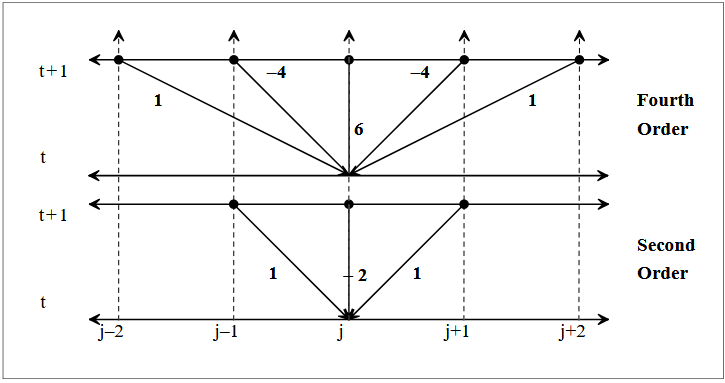
\includegraphics[width=1\textwidth]{gambar/finite_d}
	\caption{Aproksimasi turunan dengan \emph{finite differences} \citep{ivins1995everything}}
	\label{Gambar:finite_d}
\end{figure}
Turunan $\frac{\partial u^{t}_{j} }{\partial t}$ diaproksimasikan menjadi $\dfrac{ u^{t+1}_j - u^{t}_j }{\delta t}$ \citep{ivins1995everything}. Turunan orde kedua, yaitu $\frac{\partial^2 u^{t}_{j}}{\partial s^2}$ diaproksimasikan menjadi $\frac{( u^{t+1}_{j+1} + u^{t+1}_{j-1} - 2u^{t+1}_{j} )}{\delta s^2}$, sedangkan turunan orde keempat, yaitu $\frac{\partial^4 u^{t}_{j}}{\partial s^4}$ diaproksimasikan menjadi $\frac{( u^{t+1}_{j+2} - 4u^{t+1}_{j+1} + 6u^{t+1}_{j} - 4u^{t+1}_{j-1} + u^{t+1}_{j-2})}{\delta s^4}$.
Turunan dalam persamaan (\ref{snake_euler_t_partial_u}) yang diaproksimasi menggunakan \emph{finite differences} seperti yang ditunjukkan pada Gambar (\ref{Gambar:finite_d}) adalah sebagai berikut:

\begin{multline}
	\label{aprox_finite}
	\dfrac{ u^{t+1}_j - u^{t}_j }{\delta t} = \frac{\alpha}{\delta s^2}( u^{t+1}_{j+1} + u^{t+1}_{j-1} - 2u^{t+1}_{j} ) \\
	- \frac{\beta}{\delta s^4}( u^{t+1}_{j+2} - 4u^{t+1}_{j+1} + 6u^{t+1}_{j} - 4u^{t+1}_{j-1} + u^{t+1}_{j-2}) + \frac{\partial E^{(i)}_{ext} }{ \partial u^{t}_{j}}
\end{multline}

\begin{comment}
\begin{multline}
	\label{aprox_finite1}
	u^{t+1}_j - u^{t}_j = \frac{\alpha \delta t}{\delta s^2} u^{t+1}_{j+1} + \frac{\alpha \delta t}{\delta s^2} u^{t+1}_{j-1} - \frac{\alpha \delta t}{\delta s^2} 2u^{t+1}_{j} \\
	- \frac{\beta \delta t}{\delta s^4} u^{t+1}_{j+2} + \frac{\beta \delta t}{\delta s^4} 4u^{t+1}_{j+1} - \frac{\beta \delta t}{\delta s^4} 6u^{t+1}_{j} + \frac{\beta \delta t}{\delta s^4} 4u^{t+1}_{j-1} - \frac{\beta \delta t}{\delta s^4} u^{t+1}_{j-2} - \frac{\partial E^{(i)}_{ext} \delta t}{ \partial u^{t}_{j}}
\end{multline}

\begin{multline}
	\label{aprox_finite2}
	u^{t+1}_j - u^{t}_j = \frac{\alpha \delta t}{\delta s^2} u^{t+1}_{j+1} + \frac{\alpha \delta t}{\delta s^2} u^{t+1}_{j-1} - \frac{\alpha \delta t}{\delta s^2} 2u^{t+1}_{j} \\
	- \frac{\beta \delta t}{\delta s^4} u^{t+1}_{j+2} + \frac{\beta \delta t}{\delta s^4} 4u^{t+1}_{j+1} - \frac{\beta \delta t}{\delta s^4} 6u^{t+1}_{j} + \frac{\beta \delta t}{\delta s^4} 4u^{t+1}_{j-1} - \frac{\beta \delta t}{\delta s^4} u^{t+1}_{j-2} - \frac{\partial E^{(i)}_{ext} \delta t}{ \partial u^{t}_{j}}
\end{multline}
\end{comment}


di mana $t$ dan $t+1$ mewakili parameter waktu yang berurutan dengan langkah waktu (\emph{time step}) $\delta t$. $\delta s$ mewakili ukuran langkah (\emph{step size}). Mememindahkan $\delta t$ ke ruas kanan persamaan membuat persamaan (\ref{aprox_finite}) menjadi:
\begin{multline}
	\label{aprox_finite_LHS}
	b u^{t+1}_{j+2} - (a+4b) u^{t+1}_{j+1} + (1+2a+6b) u^{t+1}_{j} - (a+4b) u^{t+1}_{j-1} + b u^{t+1}_{j-2} \\
	= u^{t}_{j} + \delta t \frac{\partial E^{(i)}_{ext} }{ \partial u^{t}_{j}}
\end{multline}
di mana $a \equiv \alpha \frac{\delta t}{\delta s^2} $ dan $b \equiv \beta \frac{\delta t}{\delta s^4} $.
Persamaan (\ref{aprox_finite_LHS}) dapat juga ditulis sebagai berikut:
\begin{equation}
	\label{aprox_finite_rhs}
	p u^{t+1}_{j+2} + q u^{t+1}_{j+1} + r u^{t+1}_{j} + q u^{t+1}_{j-1} + p u^{t+1}_{j-2} \\
	= \tilde{u}^{t+1}_{j}
\end{equation}
di mana $p \equiv b$, $q \equiv -a-4b$, dan $r \equiv 1+2a+6b$, sedangkan $\tilde{u}^{t+1}_{j} = u^{t}_{j} + \delta t \frac{\partial E^{(i)}_{ext} }{ \partial u^{t}_{j}}$. Persamaan (\ref{aprox_finite_rhs}) ini dapat ditulis dalam bentuk matriks untuk koordinat $x$ dan $y$ dari setiap elemen kurva \emph{snake} $\textbf{v}$.



\begin{equation}
	\label{matriks_implicit}
	{
		\begin{bmatrix}
			r 	& q			& p 	 & 		  & 	   & p 		& q \\
			q 	& r     	& q 	 & 	p	  & 	   &  		& p \\
			p 	& q     	& r 	 & 	q	  & p	   &  		&  	\\
			& \ddots 	& \ddots & \ddots & \ddots & \ddots &  	\\
			&  			& p 	 & 	q	  & r	   & q 		& p \\
			p 	&  			& 	 	 & 	p	  & q	   & r 		& q \\
			q 	& p 		&  		 & 		  & p	   & q 		& r
		\end{bmatrix}
	}
	{
		\begin{bmatrix}
			u^{t+1}_{0} 	\\
			u^{t+1}_{1} 	\\
			u^{t+1}_{2} 	\\
			\vdots 			\\
			u^{t+1}_{N-3}\\
			u^{t+1}_{N-2}\\
			u^{t+1}_{N-1}
		\end{bmatrix}
	}
	{
		=
	}
	{
		\begin{bmatrix}
			\tilde{u}^{t+1}_{0} 	\\
			\tilde{u}^{t+1}_{1} 	\\
			\tilde{u}^{t+1}_{2} 	\\
			\vdots 					\\
			\tilde{u}^{t+1}_{N-3}	\\
			\tilde{u}^{t+1}_{N-2}	\\
			\tilde{u}^{t+1}_{N-1}
		\end{bmatrix}
	}
\end{equation}
di mana

\begin{equation}
	\label{matriks_m}
	{
		\textbf{M} =
	}
	{
		\begin{bmatrix}
			r 	& q			& p 	 & 		  & 	   & p 		& q \\
			q 	& r     	& q 	 & 	p	  & 	   &  		& p \\
			p 	& q     	& r 	 & 	q	  & p	   &  		&  	\\
			& \ddots 	& \ddots & \ddots & \ddots & \ddots &  	\\
			&  			& p 	 & 	q	  & r	   & q 		& p \\
			p 	&  			& 	 	 & 	p	  & q	   & r 		& q \\
			q 	& p 		&  		 & 		  & p	   & q 		& r
		\end{bmatrix}
	}
\end{equation}

\begin{equation}
	\label{matriks_ut1}
	{
		\textbf{u}^{t+1}_{j} =
	}
	{
		\begin{bmatrix}
			u^{t+1}_{0} 	\\
			u^{t+1}_{1} 	\\
			u^{t+1}_{2} 	\\
			\vdots 			\\
			u^{t+1}_{N-3}\\
			u^{t+1}_{N-2}\\
			u^{t+1}_{N-1}
		\end{bmatrix}
	}
\end{equation}

\begin{equation}
	\label{matriks_ut2}
	{
		\tilde{\textbf{u}}_{j}^{t+1} =
	}
	{
		\begin{bmatrix}
			\tilde{u}^{t+1}_{0} 	\\
			\tilde{u}^{t+1}_{1} 	\\
			\tilde{u}^{t+1}_{2} 	\\
			\vdots 					\\
			\tilde{u}^{t+1}_{N-3}	\\
			\tilde{u}^{t+1}_{N-2}	\\
			\tilde{u}^{t+1}_{N-1}
		\end{bmatrix}
	}
	{
		=
	}
	{
		\begin{bmatrix}
			u^{t}_{0} + \delta t \frac{\partial E^{(i)}_{ext} }{ \partial u^{t}_{0}} 	\\
			u^{t}_{1} + \delta t \frac{\partial E^{(i)}_{ext} }{ \partial u^{t}_{1}} 	\\
			u^{t}_{2} + \delta t \frac{\partial E^{(i)}_{ext} }{ \partial u^{t}_{2}} 	\\
			\vdots 					\\
			u^{t}_{N-3} + \delta t \frac{\partial E^{(i)}_{ext} }{ \partial u^{t}_{N-3}}	\\
			u^{t}_{N-2} + \delta t \frac{\partial E^{(i)}_{ext} }{ \partial u^{t}_{N-2}}	\\
			u^{t}_{N-1} + \delta t \frac{\partial E^{(i)}_{ext} }{ \partial u^{t}_{N-1}}
		\end{bmatrix}
	}
	%{
	%	=
	%}
	%{
	%	u^{t}_{j} - \delta t \frac{\partial E^{(i)}_{ext} }{ \partial u^{t}_{j}}
	%}
\end{equation}

\begin{equation}
	\label{consteq}
	p \equiv \beta \frac{\delta t}{\delta s^4}, q \equiv - \alpha \frac{\delta t}{\delta s^2} - 4 \beta \frac{\delta t}{\delta s^4}, r \equiv  1 + 2 \alpha \frac{\delta t}{\delta s^2} + 6 \beta \frac{\delta t}{\delta s^4}
\end{equation}
Mengalikan kedua sisi dari persamaan (\ref{matriks_implicit}) dengan inverse dari matriks $\textbf{M}$ memberikan solusi akhir persamaan \emph{snake} menjadi:
\begin{equation}
	\label{implicit}
	\textbf{u}^{t+1}_{j} = \textbf{M}^{-1} \biggl( \textbf{u}^t_{j} + \delta t  \frac{\partial E^{(i)}_{ext} }{ \partial \textbf{u}^{t}_{j}} \biggr)
\end{equation}

Perlu diingat $\textbf{u}$ adalah komponen/elemen $x$ dan $y$ pada kurva \emph{snake}, komponen/elemen ini dapat dinyatakan dengan vektor $\textbf{x}$ dan $\textbf{y}$. Jika $E^{(i)}_{ext}$ dinotasikan menjadi fungsi $\textbf{f}$ maka :
\begin{equation}
	\label{ext_f}
	\frac{\partial E^{(i)}_{ext} }{ \partial \textbf{u}^{t}_{j}} = \frac{\partial \textbf{f} }{ \partial \textbf{u}^{t}_{j}}
\end{equation}

Hal ini membuat persamaan (\ref{implicit}) dapat ditulis sebagai berikut:
\begin{equation}
	\label{implicit_x}
	\textbf{x}^{t+1}_{j} = \textbf{M}^{-1} \biggl( \textbf{x}^t_{j} + \delta t \; \textbf{f}_{x} \biggr)
\end{equation}
dan
\begin{equation}
	\label{implicit_y}
	\textbf{y}^{t+1}_{j} = \textbf{M}^{-1} \biggl( \textbf{y}^t_{j} + \delta t \; \textbf{f}_{y} \biggr)
\end{equation}

$\textbf{f}_x$ dan $\textbf{f}_y$ adalah vektor-vektor yang bersesuaian dengan bentuk turunan pertama $\frac{\partial \textbf{f} }{ \partial \textbf{u}^{t}_{j}}$ sebagai berikut:
\begin{equation}
	\label{fx_eq}
	% \textbf{f}_x = f_x(x^t_{j}, y^t_{j}) = f(x^t_{j}+1) , y^t_{j}) - f(x^t_{j},y^t_{j})
	\textbf{f}_x = f_x(x^t_{j}, y^t_{j})
\end{equation}

\begin{equation}
	\label{fy_eq}
	% \textbf{f}_y = f_y(x^t_{j}, y^t_{j}) = f(x^t_{j}, y^t_{j}+1) - f(x^t_{j},y^t_{j})
	\textbf{f}_y = f_y(x^t_{j}, y^t_{j})
\end{equation}
di mana $x^t_{j}$ dan $y^t_{j}$ adalah pasangan koordinat dari kurva \emph{snake}. $\textbf{f}_x$ dan $\textbf{f}_y$ dapat dicari menggunakan teori gradien citra.
%--algoritma ,equilibrium--

\section{Interpolasi Bilinear}
Interpolasi Bilinear adalah metode interpolasi fungsi dari dua variabel (misal $x$ dan $y$). Metode ini biasanya digunakan untuk mengaproksimasi nilai data di antara beberapa titik dalam \emph{2D rectangular grid}, misalnya di dalam matriks \citep{william1997numerical}.

Misal kita ingin mencari nilai fungsi $f$ yang tidak diketahui di titik $(x,y)$ dan diasumsikan kita mengetahui nilai $f$ pada beberapa empat titik $Q_11 = (x_1, y_1), Q_12 = (x_1, y_2), Q_21 = (x_2, y_1), dan Q_22 = (x_2, y_2)$ maka langkah yang harus dilakukan sebagai berikut:
\begin{equation}
	\label{bilin_x1}
	f(x,y_1) = \frac{x_2 - x}{x_2 - x1} f(Q_11) + \frac{x - x_1}{x_2 - x_1} f(Q_21) = R1
\end{equation}

\begin{equation}
	\label{bilin_x2}
	f(x,y_2) = \frac{x_2 - x}{x_2 - x1} f(Q_12) + \frac{x - x_1}{x_2 - x_1} f(Q_22) = R2
\end{equation}

\begin{equation}
	\label{bilin_y}
	f(x,y) = \frac{y_2 - y}{y_2 - y_1} f(x, y_1) + \frac{y - y_1}{y_2 - y_1} f(x, y_2) = P
\end{equation}

\begin{figure}[H]
	\centering
	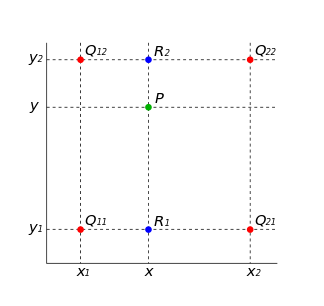
\includegraphics[width=.7\textwidth]{gambar/bilinear_interpolation}
	\caption{interpolasi bilinear}
	\label{Gambar:bilin_ilust}
\end{figure}


\begin{comment}

\section{\emph{Gradient Vector Flow (GVF) snake}}
Model \emph{snake} tradisional memiliki kekurangan seperti yang dibahas sebelumnya. Sebagian besar alasan kinerja yang buruk dikaitkan dengan energi eksternal. Untuk memperbaiki masalah ini, \citep{xu1998snakes:22} mengusulkan energi eksternal baru yang dikenal sebagai GVF \emph{snake} . 

Model dasar GVF sama dengan persamaan \emph{snake} (\ref{snake_euler_t}), tetapi yang membedakan adalah energi eksternal $- \nabla E^{(i)}_{ext}$ yang di definisikan menjadi $\textbf{g}$ sebagai berikut:
\begin{equation}
	\label{gvf_euler_t}
	\textbf{v}_{t}(s,t) = \alpha\textbf{v}_{ss}(s,t) - \beta\textbf{v}_{ssss}(s,t) + \textbf{g}  = 0
\end{equation}
di mana $\textbf{g}(x, y) = [ u (x, y), v (x, y) ]$ adalah bidang vektor(\emph{vector field}), \emph{field} ini dapat dianggap sebagai \textbf{vektor gradien} dari citra (\emph{gray-level} atau \emph{binary edge-map}) \citep{xu1998snakes:22}.

\subsection{Peta Tepi (\emph{Edge Map})}
Langkah pertama untuk mendapatkan GVF adalah mendefinisikan fungsi \emph{edge map} $f(x,y)$ yang berasal dari citra $I(x,y)$. Kita dapat menggunakan peta tepi \emph{gray-level} atau \emph{binary} sesuai yang kita tentukan berdasarkan energi eksternal \emph{snake} dasar pada persamaan (\ref{eext1}) - (\ref{eext4}) sebagai berikut:
\begin{equation}
	\label{gvf_edge_map}
	f(x,y) = - E^{(i)}_{ext}(x,y)
\end{equation}
dengan $i = 1,2,3,4$.


%================|||||=====================



\subsection{\emph{Gradient Vector Flow}}
\emph{GVF} di definisikan sebagai vektor gradien $\textbf{g}(x,y) = [u(x,y), v(x,y)]$ yang meminimalkan fungsional energi sebagai berikut
\begin{equation}
	\label{equ_gvf}
	\varepsilon = \int \int \mu (u_x^2 + u_y^2 + v_x^2 + v_y^2) + |\nabla f|^2 |\textbf{g} - \nabla f|^2 \,\, dx dx
\end{equation}
di mana $\nabla f$ adalah gradien dari \emph{edge map}. $\mu$ adalah parameter regularisasi (\emph{regularization parameter}) yang menyesuaikan antara suku pertama dan suku kedua. Parameter $\mu$ dikenal sebagai pemulusan (\emph{smoothing term}) dan data(\emph{data term}). Nilai $\mu$ bergantung pada tingkat kebisingan(\emph{noise}) yang ada pada citra $I$, yaitu semakin tinggi \emph{noise}, nilai $\mu$ sebaiknya ditingkatkan\citep{xu1998snakes:22}.

Persamaan (\ref{equ_gvf}) bukan merupakan bentuk akhir karena masih dalam bentuk integran. Untuk mencari nilai $\textbf{g}$, dua persamaan Euler dibawah ini harus diselesaikan:
\begin{equation}
	\label{equ_gvf_a1}
	\mu {\nabla}^2 u - (u - f_x) (f_x^2 + f_y^2) = 0
\end{equation}
dan
\begin{equation}
	\label{equ_gvf_a2}
	\mu {\nabla}^2 v - (v - f_y) (f_x^2 + f_y^2) = 0
\end{equation}
dengan ${\nabla}^2$ adalah operator Laplacian. Untuk menghitung $f_x$ dan $f_y$ dapat menggunakan operator gradien umum seperti operator Sobel pada persamaan (\ref{sobel_x}) dan (\ref{sobel_y}). Kedua persamaan di atas dapat diselesaikan dengan menjadikan $u$ dan $v$ sebagai fungsi waktu $t$ sebagai berikut:
\begin{equation}
	\label{equ_gvf_b1}
	u_t(x,y,t) = \mu {\nabla}^2 u(x,y,t) - [ u(x,y,t) - f_x(x,y) ] [ f^2_x (x,y) + f_y^2(x,y) ]
\end{equation}
dan
\begin{equation}
	\label{equ_gvf_b2}
	v_t(x,y,t) = \mu {\nabla}^2 v(x,y,t) - [ v(x,y,t) - f_y(x,y) ] [ f^2_x (x,y) + f_y^2(x,y) ]
\end{equation}
Persamaan (\ref{equ_gvf_b1}) dan (\ref{equ_gvf_b2}) dapat ditulis ulang sebagai berikut :
\begin{equation}
	\label{gvf_t1}
	u_t(x,y,t) = \mu {\nabla}^2 u(x,y,t) - b(x,y) u(x,y,t) + c^1(x,y)
\end{equation}
dan
\begin{equation}
	\label{gvf_t2}
	v_t(x,y,t) = \mu {\nabla}^2 v(x,y,t) - b(x,y) u(x,y,t) + c^2(x,y)
\end{equation}
di mana
\begin{equation}
	\label{gvf_b}
	b (x,y) = f_x(x,y)^2 + f_y(x,y)^2
\end{equation}
\begin{equation}
	\label{gvf_c1}
	c^1 (x,y) = b(x,y) f_x(x,y)
\end{equation}
\begin{equation}
	\label{gvf_c2}
	c^2 (x,y) = b(x,y)f_y(x,y)
\end{equation}
Untuk solusi iteratif, atur jarak antar piksel menjadi $\Delta x$ dan $\Delta y$, dan langkah waktu(\emph{time step}) untuk setiap iterasi adalah $\Delta t$. Maka selanjutnya dapat diaproksimasikan sebagai berikut\citep{xu1998snakes:22}:
\begin{equation}
	\label{gvf_ut}
	u_t = \frac{1}{\Delta t} ( u^{t+1}_{x,y} - u^t_{x,y} )
\end{equation}
\begin{equation}
	\label{gvf_vt}
	v_t = \frac{1}{\Delta t} ( v^{t+1}_{x,y} - v^n_{x,y} )
\end{equation}
\begin{equation}
	\label{gvf_laplace_u}
	\nabla^2 u = \frac{1}{\Delta x \Delta y} ( u_{x+1,y} + u_{x,y+1} + u_{x-1,y} + u_{x,y-1} - 4u_{x,y} )
\end{equation}
\begin{equation}
	\label{gvf_laplace_v}
	\nabla^2 v = \frac{1}{\Delta x \Delta y} ( v_{x+1,y} + v_{x,y+1} + v_{x-1,y} + v_{x,y-1} - 4v_{x,y} )
\end{equation}
substitusi notasi di atas ke persamaan (\ref{gvf_t1}) dan (\ref{gvf_t2}) memberikan solusi iteratif sebagai berikut
\begin{equation}
	\label{gvfc1}
	u^{t+1}_{x,y} = (1 - b_{i,j} \Delta t) u^{t}_{x,y} + r ( u^{t}_{x+1 , y} + u^t_{x,y+1} + u^t_{x-1 , y} + u^t_{x, y-1} - 4u^t_{x, y}) + c^1_{x,y} \Delta t
\end{equation}
dan
\begin{equation}
	\label{gvfc2}
	v^{t+1}_{x,y} = (1 - b_{x,y} \Delta t) v^{t}_{x,y} + r ( v^{t}_{x+1 , y} + v^n_{x,y+1} + v^t_{x-1 , y} + v^t_{x, y-1} - 4v^t_{x, y}) + c^2_{x,y} \Delta t
\end{equation}
di mana
\begin{equation}
	\label{gvf_r}
	r = \frac{ \mu \Delta t}{\Delta x \Delta y}
\end{equation}
% Selanjutnya jika $\Delta x$, $\Delta y$ dan $\mu$ konstan, maka nilai $\Delta t$ harus memenuhi \citep{CartasAyala2011GradientVF}:
Selanjutnya jika $\Delta x$, $\Delta y$ dan $\mu$ konstan, maka nilai $\Delta t$ harus memenuhi:
\begin{equation}
	\label{gvfnot5}
	\Delta t \leq \frac{\Delta x \Delta y}{4 \mu}
\end{equation}

Selanjutnya dengan mengganti bentuk energi eksternal \emph{snake} dasar masing-masing dengan $u$ dan $v$, persamaan evolusi \emph{snake} (\ref{implicit_x}) dan (\ref{implicit_y})menjadi:
\begin{equation}
	\label{implicit_gvf_u}
	\textbf{x}^{t+1} = \textbf{M}^{-1} \biggl( \textbf{x}^t + \delta t \; u^{t+1}_{x,y} \biggr)
\end{equation}
dan
\begin{equation}
	\label{implicit_gvf_y}
	\textbf{y}^{t+1} = \textbf{M}^{-1} \biggl( \textbf{y}^t + \delta t \; v^{t+1}_{x,y} \biggr)
\end{equation}


berikut adalah ilustrasi dari GVF \emph{snake}:
\begin{figure}[H]
	\centering
	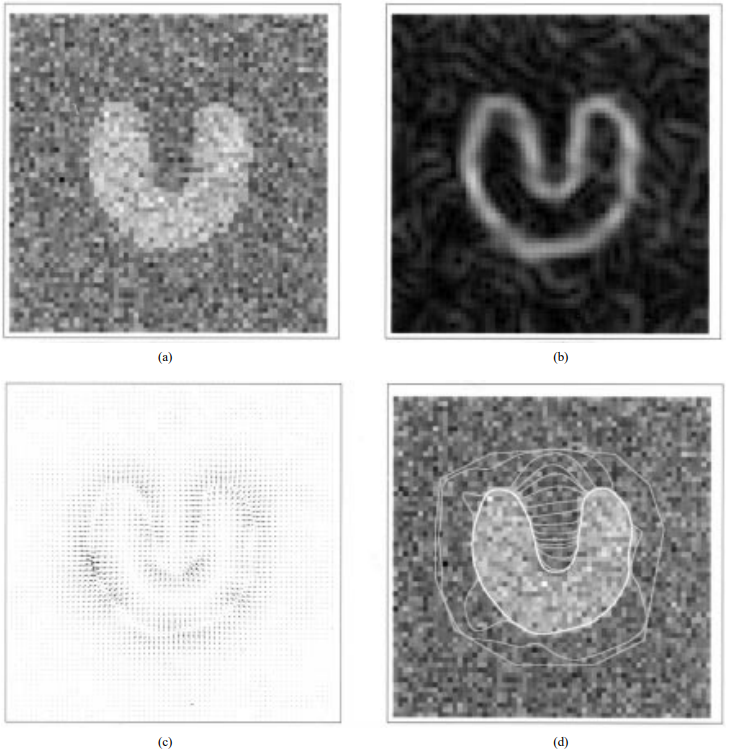
\includegraphics[width=.7\textwidth]{gambar/gvfilu}
	\caption{(a) citra objek U yang memiliki \emph{noise}; (b) \emph{edge map}; (c) medan gaya eksternal GVF; dan (d) konvergensi GVF \emph{snake} \citep{xu1998snakes:22}.}
	\label{Gambar:gvfilu}
\end{figure}

\end{comment}

% Baris ini digunakan untuk membantu dalam melakukan sitasi
% Karena diapit dengan comment, maka baris ini akan diabaikan
% oleh compiler LaTeX.
\begin{comment}
bibliography{daftar-pustaka}
\end{comment}

%!TEX root = ./template-skripsi.tex
%-------------------------------------------------------------------------------
%                            BAB III
%               			PEMBAHASAN
%-------------------------------------------------------------------------------

\chapter{METODOLOGI PENELITIAN}
Berikut ini diagram alir penelitian yang akan dilakukan:
%Selanjutnya kontur akhir akan di bandingkan dengan \emph{ground truth} menggunakan perhitungan \emph{matching similarity} antara 2 citra.
\begin{figure}[H]
	\centering
	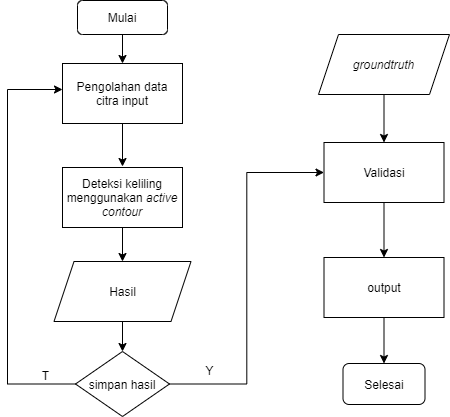
\includegraphics[width=0.6\textwidth]{diagram/metodepenelitian_alur}
	\caption{Diagram alir penelitian}
	\label{Gambar:metodepenelitian_alur}
\end{figure}

\section{Pengolahan data citra input}
Sampel yang baik adalah sampel yang mencerminkan populasinya \citep{amirullah2015metode}. Permata menggunakan data sebanyak 20 citra preparat darah pada penelitiannya tentang segmentasi parasit malaria menggunakan \emph{snake}\citep{permata2015penggunaan}, lalu pada penelitian lain Fadillah menggunakan data sebanyak 15 citra CT-Scan paru-paru pada penelitiannya tentang segmentasi citra paru-paru menggunakan \emph{snake}, dan Constantia menggunakan 21 data citra sapi dalam penelitiannya tentang estimasi bobot sapi menggunakan \emph{snake}\citep{constantia2019estimasi}. 
\begin{comment}
	Tujuan dari sebuah riset adalah untuk memperoleh informasi dari populasi. Populasi merupakan seluruh kumpulan elemen yang dapat digunakan untuk membuat kesimpulan tertentu sedangkan sampel merupakan kelompok yang dipilih dari populasi untuk digunakan dalam riset. Sampai saat ini belum ada kesepakatan atau ketentuan secara ideal dalam menentukan berapa banyak sampel dalam penelitian. 
\end{comment}

% sekaligus sebagai sampel (sampel = populasi), diujikan > tersedia
% mengurangi similarity (luka hitam 1.jpg)
% 28 -> 27 citra, 78 -> 77 citra
\emph{Dataset} luka yang penulis dapat berjumlah 108, sebanyak 37 data tidak dapat dipakai karena data tersebut memiliki duplikasi dengan data lain sehingga data yang tersedia berjumlah 71 buah citra luka yang penulis jadikan sebagai populasi sekaligus sebagai sampel penelitian (sampel = populasi) dengan kategori luka hitam sebanyak 24 citra, luka kuning sebanyak 15 citra, dan luka merah sebanyak 32 citra. \emph{Dataset} ini didapat dari penelitian luka \mbox{Ns. Ratna Aryani, M.Kep}, tahun 2018 \mbox{\citep{ratna2018rancang}} yang tersedia di \emph{repository} \url{https://github.com/mekas/InjuryDetection}. Data yang penulis gunakan adalah data-data yang berekstensi .xcf yang dapat dibuka dengan \emph{software} GIMP, pemrosesan data sebelum deteksi menggunakan \emph{snake} dan GVF dilakukan menggunakan \emph{software} GIMP. \emph{Dataset} ini masing-masing di dalamnya terdapat \emph{layer} citra (luka), \emph{layer} region (luka), dan \emph{path} sebagai berikut :
\begin{figure}[H]
	\centering
	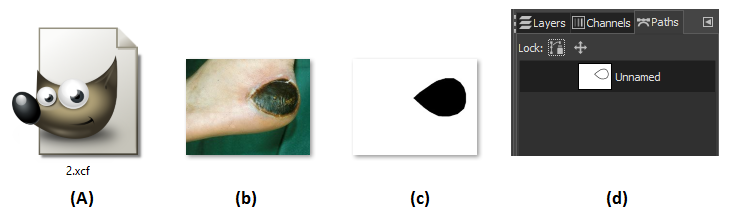
\includegraphics[width=1\textwidth]{gambar/isi_file_xcf}
	\caption{(a) Data citra format .xcf, (b) \emph{layer} citra (luka), (c) \emph{layer} region, (d) \emph{path} }
	\label{Gambar:isi_file_xcf}
\end{figure}

langkah selanjutnya adalah mengubah ukuran (\emph{resize}) citra \emph{size} yang besar ke ukuran yang lebih kecil agar proses deteksi menjadi lebih cepat. Penulis mengubah ukuran citra menggunakan fitur \emph{rescale image} sehingga ukuran citra tidak lebih dari 2 \emph{megabyte}. Kemudian penulis mengecek masing-masing citra dengan fitur \emph{eclipse select} untuk mengetahui apakah objek luka pada data citra pas berada di dalam lingkaran yang akan dijadikan sebagai inisialisasi awal. Ukuran lingkaran tidak boleh lebih besar dari ukuran citra. Jika ukuran lingkaran lebih besar daripada ukuran citra, maka perlu ditambahkan \emph{border} yang dibuat menggunakan fitur \emph{add border} sebagai berikut :
\begin{figure}[H]
	\centering
	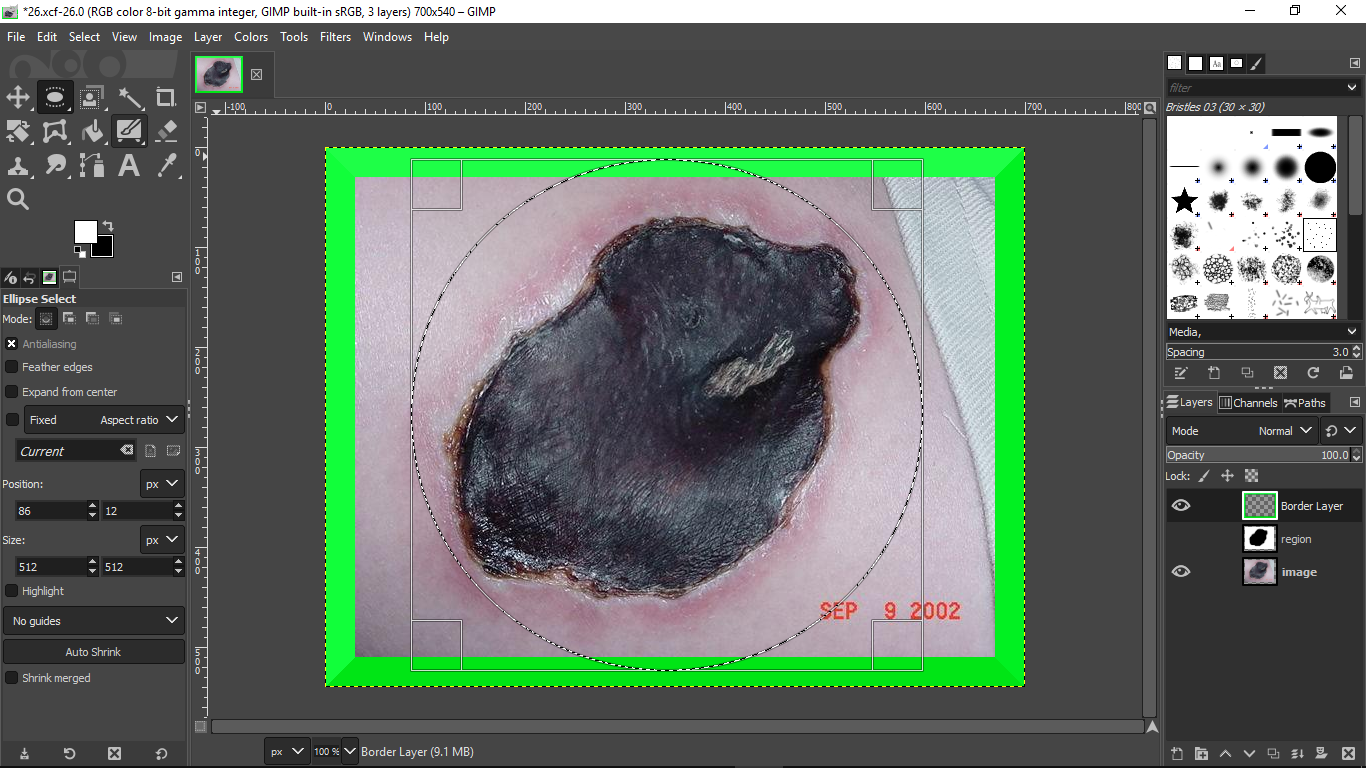
\includegraphics[width=1\textwidth]{gambar/circle_and_border}
	\caption{Citra luka yang telah dicek menggunakan fitur \emph{eclipse select} dan ditambahkan \emph{border}}
	\label{Gambar:circle_and_border}
\end{figure}

Setelah proses \emph{resize} sampai pengecekan lingkaran, selanjutnya penulis \emph{export layer} masing masing ke format .jpg.
\begin{figure}[H]
	\centering
	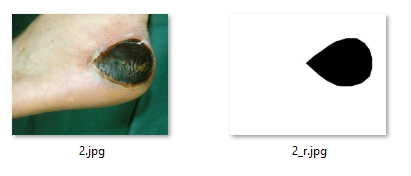
\includegraphics[width=1\textwidth]{gambar/citra_region}
	\caption{Citra luka dan region luka}
	\label{Gambar:citra_region}
\end{figure}




% checkpoint. next olah data di folder my_activecontour

\begin{comment}
\begin{table}[H]
	\centering
	\caption{Rincian data yang akan digunakan kategori luka hitam}
	\label{rinciandataset1}
	\begin{tabular}{|m{1in}|m{1in}|m{1in}|m{1in}|m{1in}|}
		\hline
		\textbf{Citra} & \textbf{\emph{Region}} & \textbf{\emph{Ground truth}} & Kurva awal & Anotasi \\
		\hline
		
		%&  &  & & \\
		%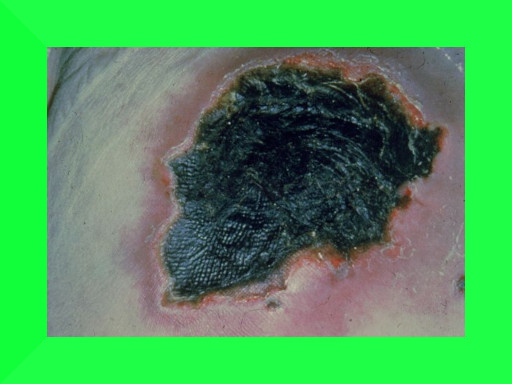
\includegraphics[width=1in]{dataset/dataset_3/luka_hitam/ready/1.jpg} 1.jpg & %
\includegraphics[width=1in]{dataset/dataset_3/luka_hitam/ready/1_r.jpg} 1\_r.jpg & %
\includegraphics[width=1in]{dataset/dataset_3/luka_hitam/ready/1_g.jpg} 1\_g.jpg &
		%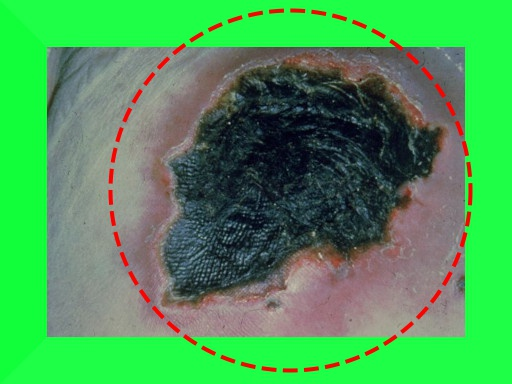
\includegraphics[width=1in]{dataset/dataset_3/luka_hitam/ready/1_init.jpg} 1\_init.jpg &
		%cr=190 
		%cc=290
		%r=180\\
		%\hline
		
		&  &  & & \\
		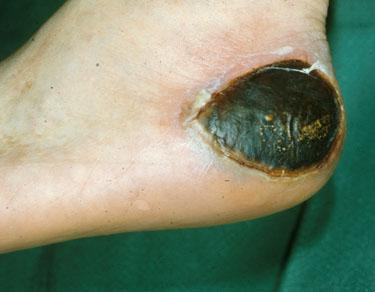
\includegraphics[width=1in]{dataset/dataset_3/luka_hitam/ready/2.jpg} 2.jpg & 
\includegraphics[width=1in]{dataset/dataset_3/luka_hitam/ready/2_r.jpg} 2\_r.jpg & 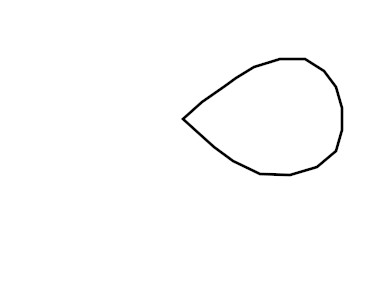
\includegraphics[width=1in]{dataset/dataset_3/luka_hitam/ready/2_g.jpg} 2\_g.jpg &
		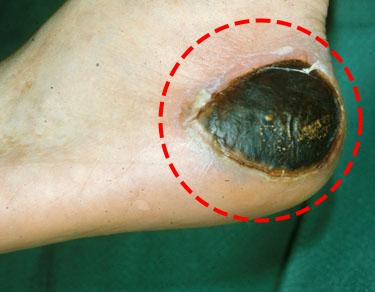
\includegraphics[width=1in]{dataset/dataset_3/luka_hitam/ready/2_init.jpg} 2\_init.jpg &
		cr=120
		cc=265
		r=85\\
		\hline
		
		&  &  & & \\
		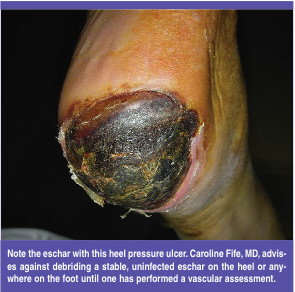
\includegraphics[width=1in]{dataset/dataset_3/luka_hitam/ready/4.jpg} 4.jpg & 
\includegraphics[width=1in]{dataset/dataset_3/luka_hitam/ready/4_r.jpg} 4\_r.jpg & 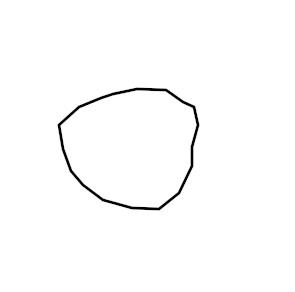
\includegraphics[width=1in]{dataset/dataset_3/luka_hitam/ready/4_g.jpg} 4\_g.jpg &
		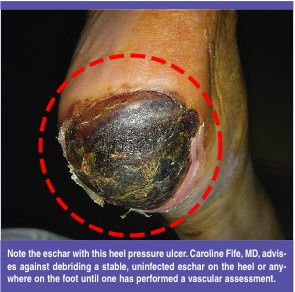
\includegraphics[width=1in]{dataset/dataset_3/luka_hitam/ready/4_init.jpg} 4\_init.jpg &
		cr=145
		cc=130
		r=90\\
		\hline
		
		&  &  & & \\
		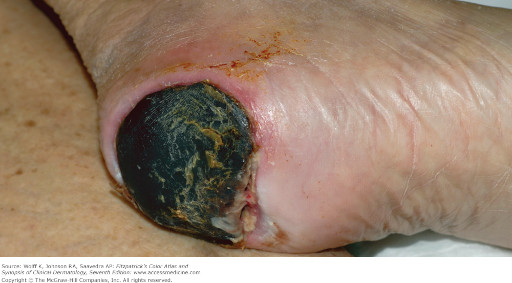
\includegraphics[width=1in]{dataset/dataset_3/luka_hitam/ready/5.jpg} 5.jpg & 
\includegraphics[width=1in]{dataset/dataset_3/luka_hitam/ready/5_r.jpg} 5\_r.jpg & 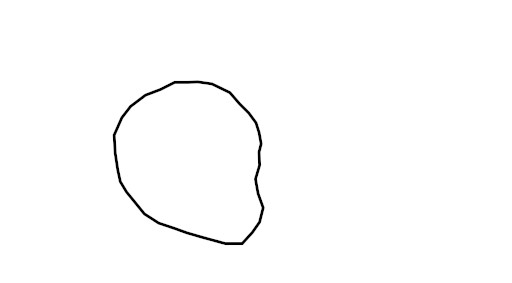
\includegraphics[width=1in]{dataset/dataset_3/luka_hitam/ready/5_g.jpg} 5\_g.jpg &
		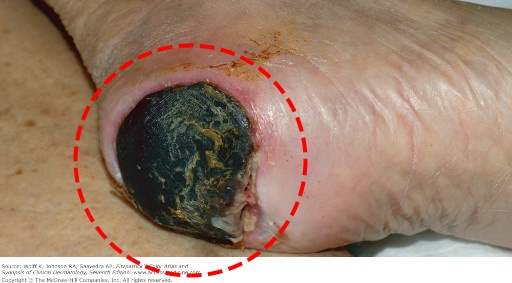
\includegraphics[width=1in]{dataset/dataset_3/luka_hitam/ready/5_init.jpg} 5\_init.jpg &
		cr=160
		cc=190
		r=115\\
		\hline
	\end{tabular}
\end{table}

\begin{table}[H]
	\centering
	\caption{Rincian data yang akan digunakan kategori luka hitam (lanjutan)}
	\label{rinciandataset2}
	\begin{tabular}{|m{1in}|m{1in}|m{1in}|m{1in}|m{1in}|}
		\hline
		\textbf{Citra} & \textbf{\emph{Region}} & \textbf{\emph{Ground truth}} & Kurva awal & Anotasi \\
		\hline
		
		&  &  & & \\
		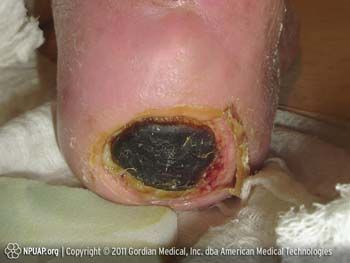
\includegraphics[width=1in]{dataset/dataset_3/luka_hitam/ready/6.jpg} 6.jpg & 
\includegraphics[width=1in]{dataset/dataset_3/luka_hitam/ready/6_r.jpg} 6\_r.jpg & 
\includegraphics[width=1in]{dataset/dataset_3/luka_hitam/ready/6_g.jpg} 6\_g.jpg &
		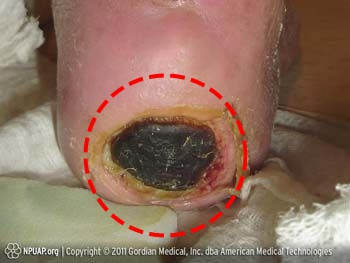
\includegraphics[width=1in]{dataset/dataset_3/luka_hitam/ready/6_init.jpg} 6\_init.jpg &
		cr=155
		cc=165
		r=80\\
		\hline
		
		&  &  & & \\
		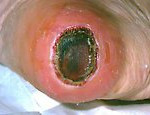
\includegraphics[width=1in]{dataset/dataset_3/luka_hitam/ready/7.jpg} 7.jpg & 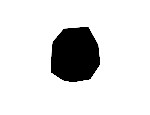
\includegraphics[width=1in]{dataset/dataset_3/luka_hitam/ready/7_r.jpg} 7\_r.jpg & 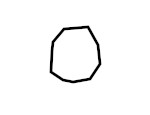
\includegraphics[width=1in]{dataset/dataset_3/luka_hitam/ready/7_g.jpg} 7\_g.jpg &
		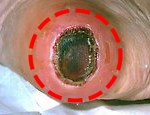
\includegraphics[width=1in]{dataset/dataset_3/luka_hitam/ready/7_init.jpg} 7\_init.jpg &
		cr=55
		cc=75
		r=45\\
		\hline
		
		&  &  & & \\
		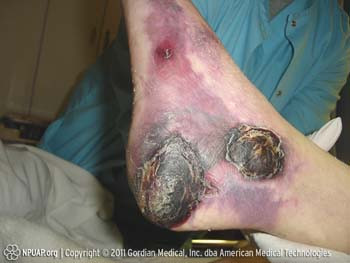
\includegraphics[width=1in]{dataset/dataset_3/luka_hitam/ready/8.jpg} 8.jpg & 
\includegraphics[width=1in]{dataset/dataset_3/luka_hitam/ready/8_r.jpg} 8\_r.jpg & 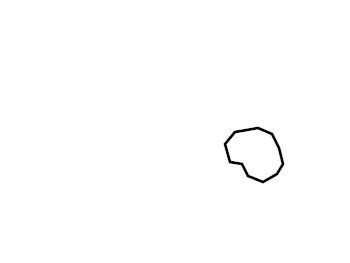
\includegraphics[width=1in]{dataset/dataset_3/luka_hitam/ready/8_g.jpg} 8\_g.jpg &
		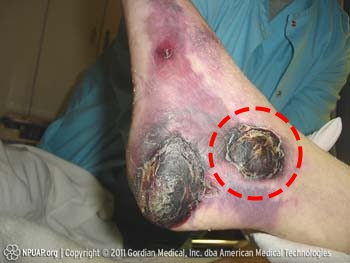
\includegraphics[width=1in]{dataset/dataset_3/luka_hitam/ready/8_init.jpg} 8\_init.jpg &
		cr=153
		cc=255
		r=45\\
		\hline
		
		&  &  & & \\
		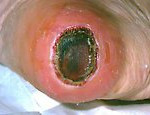
\includegraphics[width=1in]{dataset/dataset_3/luka_hitam/duplicate_or_copyright/9.jpg} 9.jpg & 
\includegraphics[width=1in]{dataset/dataset_3/luka_hitam/duplicate_or_copyright/9_r.jpg} 9\_r.jpg & 
\includegraphics[width=1in]{dataset/dataset_3/luka_hitam/duplicate_or_copyright/9_g.jpg} 9\_g.jpg &
		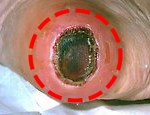
\includegraphics[width=1in]{dataset/dataset_3/luka_hitam/duplicate_or_copyright/9_init.jpg} 9\_init.jpg &
		cr=55
		cc=75
		r=45\\
		\hline
		
		&  &  & & \\
		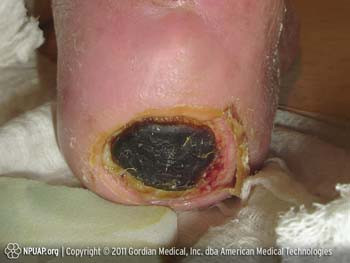
\includegraphics[width=1in]{dataset/dataset_3/luka_hitam/duplicate_or_copyright/11.jpg} 11.jpg & 
\includegraphics[width=1in]{dataset/dataset_3/luka_hitam/duplicate_or_copyright/11_r.jpg} 11\_r.jpg & 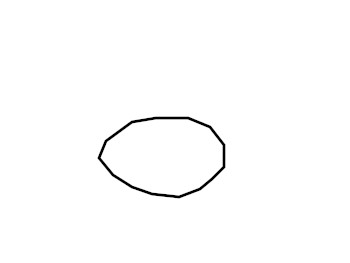
\includegraphics[width=1in]{dataset/dataset_3/luka_hitam/duplicate_or_copyright/11_g.jpg} 11\_g.jpg &
		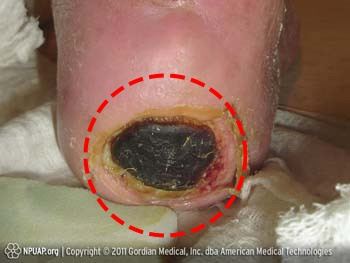
\includegraphics[width=1in]{dataset/dataset_3/luka_hitam/duplicate_or_copyright/11_init.jpg} 11\_init.jpg &
		cr=155
		cc=165
		r=80\\
		\hline
	\end{tabular}
\end{table}

\begin{table}[H]
	\centering
	\caption{Rincian data yang akan digunakan kategori luka hitam (lanjutan)}
	\label{rinciandataset3}
	\begin{tabular}{|m{1in}|m{1in}|m{1in}|m{1in}|m{1in}|}
		\hline
		\textbf{Citra} & \textbf{\emph{Region}} & \textbf{\emph{Ground truth}} & Kurva awal & Anotasi \\
		\hline
		
		&  &  & & \\
		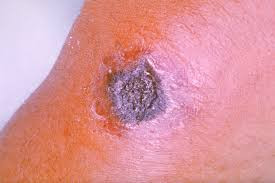
\includegraphics[width=1in]{dataset/dataset_3/luka_hitam/ready/14.jpg} 14.jpg & \includegraphics[width=1in]{dataset/dataset_3/luka_hitam/ready/14_r.jpg} 14\_r.jpg & \includegraphics[width=1in]{dataset/dataset_3/luka_hitam/ready/14_g.jpg} 14\_g.jpg &
		\includegraphics[width=1in]{dataset/dataset_3/luka_hitam/ready/14_init.jpg} 14\_init.jpg &
		cr=95
		cc=130
		r=65\\
		\hline
		
		&  &  & & \\
		\includegraphics[width=1in]{dataset/dataset_3/luka_hitam/ready/15.jpg} 15.jpg & \includegraphics[width=1in]{dataset/dataset_3/luka_hitam/ready/15_r.jpg} 15\_r.jpg & \includegraphics[width=1in]{dataset/dataset_3/luka_hitam/ready/15_g.jpg} 15\_g.jpg &
		\includegraphics[width=1in]{dataset/dataset_3/luka_hitam/ready/15_init.jpg} 15\_init.jpg &
		cr=153
		cc=250
		r=151\\
		\hline
		
		&  &  & & \\
		\includegraphics[width=1in]{dataset/dataset_3/luka_hitam/ready/16.jpg} 16.jpg & \includegraphics[width=1in]{dataset/dataset_3/luka_hitam/ready/16_r.jpg} 16\_r.jpg & \includegraphics[width=1in]{dataset/dataset_3/luka_hitam/ready/16_g.jpg} 16\_g.jpg &
		\includegraphics[width=1in]{dataset/dataset_3/luka_hitam/ready/16_init.jpg} 16\_init.jpg &
		cr=208
		cc=245
		r=200\\
		\hline
		
		&  &  & & \\
		\includegraphics[width=1in]{dataset/dataset_3/luka_hitam/ready/17.jpg} 17.jpg & \includegraphics[width=1in]{dataset/dataset_3/luka_hitam/ready/17_r.jpg} 17\_r.jpg & \includegraphics[width=1in]{dataset/dataset_3/luka_hitam/ready/17_g.jpg} 17\_g.jpg &
		\includegraphics[width=1in]{dataset/dataset_3/luka_hitam/ready/17_init.jpg} 17\_init.jpg &
		cr=124
		cc=125
		r=120\\
		\hline
		
		&  &  & & \\
		\includegraphics[width=1in]{dataset/dataset_3/luka_hitam/ready/18.jpg} 18.jpg & \includegraphics[width=1in]{dataset/dataset_3/luka_hitam/ready/18_r.jpg} 18\_r.jpg & \includegraphics[width=1in]{dataset/dataset_3/luka_hitam/ready/18_g.jpg} 18\_g.jpg &
		\includegraphics[width=1in]{dataset/dataset_3/luka_hitam/ready/18_init.jpg} 18\_init.jpg &
		cr=85
		cc=85
		r=75\\
		\hline
	\end{tabular}
\end{table}

\begin{table}[H]
	\centering
	\caption{Rincian data yang akan digunakan kategori luka hitam (lanjutan)}
	\label{rinciandataset4}
	\begin{tabular}{|m{1in}|m{1in}|m{1in}|m{1in}|m{1in}|}
		\hline
		\textbf{Citra} & \textbf{\emph{Region}} & \textbf{\emph{Ground truth}} & Kurva awal & Anotasi \\
		\hline
		
		&  &  & & \\
		\includegraphics[width=1in]{dataset/dataset_3/luka_hitam/ready/19.jpg} 19.jpg & \includegraphics[width=1in]{dataset/dataset_3/luka_hitam/ready/19_r.jpg} 19\_r.jpg & \includegraphics[width=1in]{dataset/dataset_3/luka_hitam/ready/19_g.jpg} 19\_g.jpg &
		\includegraphics[width=1in]{dataset/dataset_3/luka_hitam/ready/19_init.jpg} 19\_init.jpg &
		cr=225
		cc=285
		r=130\\
		\hline
		
		&  &  & & \\
		\includegraphics[width=1in]{dataset/dataset_3/luka_hitam/ready/20.jpg} 20.jpg & \includegraphics[width=1in]{dataset/dataset_3/luka_hitam/ready/20_r.jpg} 20\_r.jpg & \includegraphics[width=1in]{dataset/dataset_3/luka_hitam/ready/20_g.jpg} 20\_g.jpg &
		\includegraphics[width=1in]{dataset/dataset_3/luka_hitam/ready/20_init.jpg} 20\_init.jpg &
		cr=250
		cc=225
		r=155\\
		\hline
		
		&  &  & & \\
		\includegraphics[width=1in]{dataset/dataset_3/luka_hitam/ready/22.jpg} 22.jpg & \includegraphics[width=1in]{dataset/dataset_3/luka_hitam/ready/22_r.jpg} 22\_r.jpg & \includegraphics[width=1in]{dataset/dataset_3/luka_hitam/ready/22_g.jpg} 22\_g.jpg &
		\includegraphics[width=1in]{dataset/dataset_3/luka_hitam/ready/22_init.jpg} 22\_init.jpg &
		cr=140
		cc=190
		r=125\\
		\hline
		
		&  &  & & \\
		\includegraphics[width=1in]{dataset/dataset_3/luka_hitam/duplicate_or_copyright/24.jpg} 24.jpg & \includegraphics[width=1in]{dataset/dataset_3/luka_hitam/duplicate_or_copyright/24_r.jpg} 24\_r.jpg & \includegraphics[width=1in]{dataset/dataset_3/luka_hitam/duplicate_or_copyright/24_g.jpg} 24\_g.jpg &
		\includegraphics[width=1in]{dataset/dataset_3/luka_hitam/duplicate_or_copyright/24_init.jpg} 24\_init.jpg &
		cr=190
		cc=190
		r=180\\
		\hline
		
		&  &  & & \\
		\includegraphics[width=1in]{dataset/dataset_3/luka_hitam/ready/26.jpg} 26.jpg & \includegraphics[width=1in]{dataset/dataset_3/luka_hitam/ready/26_r.jpg} 26\_r.jpg & \includegraphics[width=1in]{dataset/dataset_3/luka_hitam/ready/26_g.jpg} 26\_g.jpg &
		\includegraphics[width=1in]{dataset/dataset_3/luka_hitam/ready/26_init.jpg} 26\_init.jpg &
		cr=195
		cc=248
		r=193\\
		\hline
	\end{tabular}
\end{table}

\begin{table}[H]
	\centering
	\caption{Rincian data yang akan digunakan kategori luka hitam (lanjutan)}
	\label{rinciandataset5}
	\begin{tabular}{|m{1in}|m{1in}|m{1in}|m{1in}|m{1in}|}
		\hline
		\textbf{Citra} & \textbf{\emph{Region}} & \textbf{\emph{Ground truth}} & Kurva awal & Anotasi \\
		\hline
		
		&  &  & & \\
		\includegraphics[width=1in]{dataset/dataset_3/luka_hitam/ready/27.jpg} 27.jpg & \includegraphics[width=1in]{dataset/dataset_3/luka_hitam/ready/27_r.jpg} 27\_r.jpg & \includegraphics[width=1in]{dataset/dataset_3/luka_hitam/ready/27_g.jpg} 27\_g.jpg &
		\includegraphics[width=1in]{dataset/dataset_3/luka_hitam/ready/27_init.jpg} 27\_init.jpg &
		cr=207
		cc=253
		r=205\\
		\hline
		
		&  &  & & \\
		\includegraphics[width=1in]{dataset/dataset_3/luka_hitam/ready/28.jpg} 28.jpg & \includegraphics[width=1in]{dataset/dataset_3/luka_hitam/ready/28_r.jpg} 28\_r.jpg & \includegraphics[width=1in]{dataset/dataset_3/luka_hitam/ready/28_g.jpg} 28\_g.jpg &
		\includegraphics[width=1in]{dataset/dataset_3/luka_hitam/ready/28_init.jpg} 28\_init.jpg &
		cr=120
		cc=80
		r=70\\
		\hline
		
		&  &  & & \\
		\includegraphics[width=1in]{dataset/dataset_3/luka_hitam/ready/29.jpg} 29.jpg & \includegraphics[width=1in]{dataset/dataset_3/luka_hitam/ready/29_r.jpg} 29\_r.jpg & \includegraphics[width=1in]{dataset/dataset_3/luka_hitam/ready/29_g.jpg} 29\_g.jpg &
		\includegraphics[width=1in]{dataset/dataset_3/luka_hitam/ready/16_init.jpg} 29\_init.jpg &
		cr=195
		cc=240
		r=180\\
		\hline
		
		&  &  & & \\
		\includegraphics[width=1in]{dataset/dataset_3/luka_hitam/ready/31.jpg} 31.jpg & \includegraphics[width=1in]{dataset/dataset_3/luka_hitam/ready/31_r.jpg} 31\_r.jpg & \includegraphics[width=1in]{dataset/dataset_3/luka_hitam/ready/31_g.jpg} 31\_g.jpg &
		\includegraphics[width=1in]{dataset/dataset_3/luka_hitam/ready/31_init.jpg} 31\_init.jpg &
		cr=245
		cc=190
		r=180\\
		\hline
		
		&  &  & & \\
		\includegraphics[width=1in]{dataset/dataset_3/luka_hitam/ready/33.jpg} 33.jpg & \includegraphics[width=1in]{dataset/dataset_3/luka_hitam/ready/33_r.jpg} 33\_r.jpg & \includegraphics[width=1in]{dataset/dataset_3/luka_hitam/ready/33_g.jpg} 33\_g.jpg &
		\includegraphics[width=1in]{dataset/dataset_3/luka_hitam/ready/33_init.jpg} 33\_init.jpg &
		cr=120
		cc=195
		r=100\\
		\hline
	\end{tabular}
\end{table}

\begin{table}[H]
	\centering
	\caption{Rincian data yang akan digunakan kategori luka hitam (lanjutan)}
	\label{rinciandataset6}
	\begin{tabular}{|m{1in}|m{1in}|m{1in}|m{1in}|m{1in}|}
		\hline
		\textbf{Citra} & \textbf{\emph{Region}} & \textbf{\emph{Ground truth}} & Kurva awal & Anotasi \\
		\hline
		
		&  &  & & \\
		\includegraphics[width=1in]{dataset/dataset_3/luka_hitam/ready/37.jpg} 37.jpg & \includegraphics[width=1in]{dataset/dataset_3/luka_hitam/ready/37_r.jpg} 37\_r.jpg & \includegraphics[width=1in]{dataset/dataset_3/luka_hitam/ready/37_g.jpg} 37\_g.jpg &
		\includegraphics[width=1in]{dataset/dataset_3/luka_hitam/ready/37_init.jpg} 37\_init.jpg &
		cr=110
		cc=125
		r=95\\
		\hline
		
		&  &  & & \\
		\includegraphics[width=1in]{dataset/dataset_3/luka_hitam/ready/39.jpg} 39.jpg & \includegraphics[width=1in]{dataset/dataset_3/luka_hitam/ready/39_r.jpg} 39\_r.jpg & \includegraphics[width=1in]{dataset/dataset_3/luka_hitam/ready/39_g.jpg} 39\_g.jpg &
		\includegraphics[width=1in]{dataset/dataset_3/luka_hitam/ready/39_init.jpg} 39\_init.jpg &
		cr=260
		cc=265
		r=170\\
		\hline
		
		&  &  & & \\
		\includegraphics[width=1in]{dataset/dataset_3/luka_hitam/ready/40.jpg} 40.jpg & \includegraphics[width=1in]{dataset/dataset_3/luka_hitam/ready/40_r.jpg} 40\_r.jpg & \includegraphics[width=1in]{dataset/dataset_3/luka_hitam/ready/40_g.jpg} 40\_g.jpg &
		\includegraphics[width=1in]{dataset/dataset_3/luka_hitam/ready/40_init.jpg} 40\_init.jpg &
		cr=90
		cc=100
		r=65\\
		\hline
		
		&  &  & & \\
		\includegraphics[width=1in]{dataset/dataset_3/luka_hitam/ready/41.jpg} 41.jpg & \includegraphics[width=1in]{dataset/dataset_3/luka_hitam/ready/41_r.jpg} 41\_r.jpg & \includegraphics[width=1in]{dataset/dataset_3/luka_hitam/ready/41_g.jpg} 41\_g.jpg &
		\includegraphics[width=1in]{dataset/dataset_3/luka_hitam/ready/41_init.jpg} 41\_init.jpg &
		cr=105
		cc=170
		r=100\\
		\hline
	\end{tabular}
\end{table}


\begin{table}[H]
	\centering
	\caption{Rincian data yang akan digunakan kategori luka kuning}
	\label{rinciandataset7}
	\begin{tabular}{|m{1in}|m{1in}|m{1in}|m{1in}|m{1in}|}
		\hline
		\textbf{Citra} & \textbf{\emph{Region}} & \textbf{\emph{Ground truth}} & Kurva awal & Anotasi \\
		\hline
		
		&  &  & & \\
		\includegraphics[width=1in]{dataset/dataset_3/luka_kuning/ready/3.jpg} 3.jpg & \includegraphics[width=1in]{dataset/dataset_3/luka_kuning/ready/3_r.jpg} 3\_r.jpg & \includegraphics[width=1in]{dataset/dataset_3/luka_kuning/ready/3_g.jpg} 3\_g.jpg &
		\includegraphics[width=1in]{dataset/dataset_3/luka_kuning/ready/3_init.jpg} 3\_init.jpg &
		cr=80
		cc=85
		r=65\\
		\hline
		
		&  &  & & \\
		\includegraphics[width=1in]{dataset/dataset_3/luka_kuning/ready/10.jpg} 10.jpg & \includegraphics[width=1in]{dataset/dataset_3/luka_kuning/ready/10_r.jpg} 10\_r.jpg & \includegraphics[width=1in]{dataset/dataset_3/luka_kuning/ready/10_g.jpg} 10\_g.jpg &
		\includegraphics[width=1in]{dataset/dataset_3/luka_kuning/ready/10_init.jpg} 10\_init.jpg &
		cr=155
		cc=133
		r=128\\
		\hline
		
		&  &  & & \\
		\includegraphics[width=1in]{dataset/dataset_3/luka_kuning/ready/12.jpg} 12.jpg & \includegraphics[width=1in]{dataset/dataset_3/luka_kuning/ready/12_r.jpg} 12\_r.jpg & \includegraphics[width=1in]{dataset/dataset_3/luka_kuning/ready/12_g.jpg} 12\_g.jpg &
		\includegraphics[width=1in]{dataset/dataset_3/luka_kuning/ready/12_init.jpg} 12\_init.jpg &
		cr=90
		cc=138
		r=70\\
		\hline
		
		&  &  & & \\
		\includegraphics[width=1in]{dataset/dataset_3/luka_kuning/ready/13.jpg} 13.jpg & \includegraphics[width=1in]{dataset/dataset_3/luka_kuning/ready/13_r.jpg} 13\_r.jpg & \includegraphics[width=1in]{dataset/dataset_3/luka_kuning/ready/13_g.jpg} 13\_g.jpg &
		\includegraphics[width=1in]{dataset/dataset_3/luka_kuning/ready/13_init.jpg} 13\_init.jpg &
		cr=70
		cc=206
		r=50\\
		\hline
		
		&  &  & & \\
		\includegraphics[width=1in]{dataset/dataset_3/luka_kuning/ready/16.jpg} 16.jpg & \includegraphics[width=1in]{dataset/dataset_3/luka_kuning/ready/16_r.jpg} 16\_r.jpg & \includegraphics[width=1in]{dataset/dataset_3/luka_kuning/ready/16_g.jpg} 16\_g.jpg &
		\includegraphics[width=1in]{dataset/dataset_3/luka_kuning/ready/16_init.jpg} 16\_init.jpg &
		cr=135
		cc=172
		r=130\\
		\hline
	\end{tabular}
\end{table}

\begin{table}[H]
	\centering
	\caption{Rincian data yang akan digunakan kategori luka kuning (lanjutan)}
	\label{rinciandataset8}
	\begin{tabular}{|m{1in}|m{1in}|m{1in}|m{1in}|m{1in}|}
		\hline
		\textbf{Citra} & \textbf{\emph{Region}} & \textbf{\emph{Ground truth}} & Kurva awal & Anotasi \\
		\hline
		
		&  &  & & \\
		\includegraphics[width=1in]{dataset/dataset_3/luka_kuning/ready/17.jpg} 17.jpg & \includegraphics[width=1in]{dataset/dataset_3/luka_kuning/ready/17_r.jpg} 17\_r.jpg & \includegraphics[width=1in]{dataset/dataset_3/luka_kuning/ready/17_g.jpg} 17\_g.jpg &
		\includegraphics[width=1in]{dataset/dataset_3/luka_kuning/ready/17_init.jpg} 17\_init.jpg &
		cr=125
		cc=115
		r=25\\
		\hline
		
		&  &  & & \\
		\includegraphics[width=1in]{dataset/dataset_3/luka_kuning/ready/18.jpg} 18.jpg & \includegraphics[width=1in]{dataset/dataset_3/luka_kuning/ready/18_r.jpg} 18\_r.jpg & \includegraphics[width=1in]{dataset/dataset_3/luka_kuning/ready/18_g.jpg} 18\_g.jpg &
		\includegraphics[width=1in]{dataset/dataset_3/luka_kuning/ready/18_init.jpg} 18\_init.jpg &
		cr=95
		cc=130
		r=80\\
		\hline
		
		&  &  & & \\
		\includegraphics[width=1in]{dataset/dataset_3/luka_kuning/ready/19.jpg} 19.jpg & \includegraphics[width=1in]{dataset/dataset_3/luka_kuning/ready/19_r.jpg} 19\_r.jpg & \includegraphics[width=1in]{dataset/dataset_3/luka_kuning/ready/19_g.jpg} 19\_g.jpg &
		\includegraphics[width=1in]{dataset/dataset_3/luka_kuning/ready/19_init.jpg} 19\_init.jpg &
		cr=60
		cc=60
		r=50\\
		\hline
		
		&  &  & & \\
		\includegraphics[width=1in]{dataset/dataset_3/luka_kuning/ready/21.jpg} 21.jpg & \includegraphics[width=1in]{dataset/dataset_3/luka_kuning/ready/21_r.jpg} 21\_r.jpg & \includegraphics[width=1in]{dataset/dataset_3/luka_kuning/ready/21_g.jpg} 21\_g.jpg &
		\includegraphics[width=1in]{dataset/dataset_3/luka_kuning/ready/21_init.jpg} 21\_init.jpg &
		cr=130
		cc=170
		r=70\\
		\hline
		
		&  &  & & \\
		\includegraphics[width=1in]{dataset/dataset_3/luka_kuning/ready/23.jpg} 23.jpg & \includegraphics[width=1in]{dataset/dataset_3/luka_kuning/ready/23_r.jpg} 23\_r.jpg & \includegraphics[width=1in]{dataset/dataset_3/luka_kuning/ready/23_g.jpg} 23\_g.jpg &
		\includegraphics[width=1in]{dataset/dataset_3/luka_kuning/ready/23_init.jpg} 23\_init.jpg &
		cr=170
		cc=230
		r=160\\
		\hline
	\end{tabular}
\end{table}

\begin{table}[H]
	\centering
	\caption{Rincian data yang akan digunakan kategori luka kuning (lanjutan)}
	\label{rinciandataset9}
	\begin{tabular}{|m{1in}|m{1in}|m{1in}|m{1in}|m{1in}|}
		\hline
		\textbf{Citra} & \textbf{\emph{Region}} & \textbf{\emph{Ground truth}} & Kurva awal & Anotasi \\
		\hline
		
		&  &  & & \\
		\includegraphics[width=1in]{dataset/dataset_3/luka_kuning/ready/25.jpg} 25.jpg & \includegraphics[width=1in]{dataset/dataset_3/luka_kuning/ready/25_r.jpg} 25\_r.jpg & \includegraphics[width=1in]{dataset/dataset_3/luka_kuning/ready/25_g.jpg} 25\_g.jpg &
		\includegraphics[width=1in]{dataset/dataset_3/luka_kuning/ready/25_init.jpg} 25\_init.jpg &
		cr=145
		cc=130
		r=55\\
		\hline
		
		&  &  & & \\
		\includegraphics[width=1in]{dataset/dataset_3/luka_kuning/ready/34.jpg} 34.jpg & \includegraphics[width=1in]{dataset/dataset_3/luka_kuning/ready/34_r.jpg} 34\_r.jpg & \includegraphics[width=1in]{dataset/dataset_3/luka_kuning/ready/34_g.jpg} 34\_g.jpg &
		\includegraphics[width=1in]{dataset/dataset_3/luka_kuning/ready/34_init.jpg} 34\_init.jpg &
		cr=185
		cc=245
		r=130\\
		\hline
		
		&  &  & & \\
		\includegraphics[width=1in]{dataset/dataset_3/luka_kuning/ready/35.jpg} 35.jpg & \includegraphics[width=1in]{dataset/dataset_3/luka_kuning/ready/35_r.jpg} 35\_r.jpg & \includegraphics[width=1in]{dataset/dataset_3/luka_kuning/ready/35_g.jpg} 35\_g.jpg &
		\includegraphics[width=1in]{dataset/dataset_3/luka_kuning/ready/35_init.jpg} 35\_init.jpg &
		cr=105
		cc=110
		r=100\\
		\hline
		
		&  &  & & \\
		\includegraphics[width=1in]{dataset/dataset_3/luka_kuning/ready/38.jpg} 38.jpg & \includegraphics[width=1in]{dataset/dataset_3/luka_kuning/ready/38_r.jpg} 38\_r.jpg & \includegraphics[width=1in]{dataset/dataset_3/luka_kuning/ready/38_g.jpg} 38\_g.jpg &
		\includegraphics[width=1in]{dataset/dataset_3/luka_kuning/ready/38_init.jpg} 38\_init.jpg &
		cr=150
		cc=280
		r=120\\
		\hline
		
		&  &  & & \\
		\includegraphics[width=1in]{dataset/dataset_3/luka_kuning/ready/42.jpg} 42.jpg & \includegraphics[width=1in]{dataset/dataset_3/luka_kuning/ready/42_r.jpg} 42\_r.jpg & \includegraphics[width=1in]{dataset/dataset_3/luka_kuning/ready/42_g.jpg} 42\_g.jpg &
		\includegraphics[width=1in]{dataset/dataset_3/luka_kuning/ready/42_init.jpg} 42\_init.jpg &
		cr=160
		cc=260
		r=1135\\
		\hline
	\end{tabular}
\end{table}


\begin{table}[H]
	\centering
	\caption{Rincian data yang akan digunakan kategori luka merah }
	\label{rinciandataset10}
	\begin{tabular}{|m{1in}|m{1in}|m{1in}|m{1in}|m{1in}|}
		\hline
		\textbf{Citra} & \textbf{\emph{Region}} & \textbf{\emph{Ground truth}} & Kurva awal & Anotasi \\
		\hline
		
		&  &  & & \\
		\includegraphics[width=0.8in]{dataset/dataset_3/luka_merah/ready/1.jpg} 1.jpg & \includegraphics[width=0.8in]{dataset/dataset_3/luka_merah/ready/1_r.jpg} 1\_r.jpg & \includegraphics[width=0.8in]{dataset/dataset_3/luka_merah/ready/1_g.jpg} 1\_g.jpg &
		\includegraphics[width=0.8in]{dataset/dataset_3/luka_merah/ready/1_init.jpg} 1\_init.jpg &
		cr=200
		cc=235
		r=190\\
		\hline
		
		&  &  & & \\
		\includegraphics[width=0.8in]{dataset/dataset_3/luka_merah/ready/2.jpg} 2.jpg & \includegraphics[width=0.8in]{dataset/dataset_3/luka_merah/ready/2_r.jpg} 2\_r.jpg & \includegraphics[width=0.8in]{dataset/dataset_3/luka_merah/ready/2_g.jpg} 2\_g.jpg &
		\includegraphics[width=0.8in]{dataset/dataset_3/luka_merah/ready/2_init.jpg} 2\_init.jpg &
		cr=270
		cc=105
		r=100\\
		\hline
		
		&  &  & & \\
		\includegraphics[width=0.8in]{dataset/dataset_3/luka_merah/ready/3.jpg} 3.jpg & \includegraphics[width=0.8in]{dataset/dataset_3/luka_merah/ready/3_r.jpg} 3\_r.jpg & \includegraphics[width=0.8in]{dataset/dataset_3/luka_merah/ready/3_g.jpg} 3\_g.jpg &
		\includegraphics[width=0.8in]{dataset/dataset_3/luka_merah/ready/3_init.jpg} 3\_init.jpg &
		cr=255
		cc=170
		r=100\\
		\hline
		
		&  &  & & \\
		\includegraphics[width=0.8in]{dataset/dataset_3/luka_merah/ready/4.jpg} 4.jpg & \includegraphics[width=0.8in]{dataset/dataset_3/luka_merah/ready/4_r.jpg} 4\_r.jpg & \includegraphics[width=0.8in]{dataset/dataset_3/luka_merah/ready/4_g.jpg} 4\_g.jpg &
		\includegraphics[width=0.8in]{dataset/dataset_3/luka_merah/ready/4_init.jpg} 4\_init.jpg &
		cr=310
		cc=170
		r=150\\
		\hline
		
		&  &  & & \\
		\includegraphics[width=0.8in]{dataset/dataset_3/luka_merah/ready/6.jpg} 6.jpg & \includegraphics[width=0.8in]{dataset/dataset_3/luka_merah/ready/6_r.jpg} 6\_r.jpg & \includegraphics[width=0.8in]{dataset/dataset_3/luka_merah/ready/6_g.jpg} 6\_g.jpg &
		\includegraphics[width=0.8in]{dataset/dataset_3/luka_merah/ready/6_init.jpg} 6\_init.jpg &
		cr=160
		cc=250
		r=120\\
		\hline
	\end{tabular}
\end{table}

\begin{table}[H]
	\centering
	\caption{Rincian data yang akan digunakan kategori luka merah (lanjutan)}
	\label{rinciandataset11}
	\begin{tabular}{|m{1in}|m{1in}|m{1in}|m{1in}|m{1in}|}
		\hline
		\textbf{Citra} & \textbf{\emph{Region}} & \textbf{\emph{Ground truth}} & Kurva awal & Anotasi \\
		\hline
		
		&  &  & & \\
		\includegraphics[width=1in]{dataset/dataset_3/luka_merah/ready/7.jpg} 7.jpg & \includegraphics[width=1in]{dataset/dataset_3/luka_merah/ready/7_r.jpg} 7\_r.jpg & \includegraphics[width=1in]{dataset/dataset_3/luka_merah/ready/7_g.jpg} 7\_g.jpg &
		\includegraphics[width=1in]{dataset/dataset_3/luka_merah/ready/7_init.jpg} 7\_init.jpg &
		cr=180
		cc=250
		r=90\\
		\hline
		
		&  &  & & \\
		\includegraphics[width=1in]{dataset/dataset_3/luka_merah/ready/8.jpg} 8.jpg & \includegraphics[width=1in]{dataset/dataset_3/luka_merah/ready/8_r.jpg} 8\_r.jpg & \includegraphics[width=1in]{dataset/dataset_3/luka_merah/ready/8_g.jpg} 8\_g.jpg &
		\includegraphics[width=1in]{dataset/dataset_3/luka_merah/ready/8_init.jpg} 8\_init.jpg &
		cr=220
		cc=260
		r=140\\
		\hline
		
		&  &  & & \\
		\includegraphics[width=1in]{dataset/dataset_3/luka_merah/ready/9.jpg} 9.jpg & \includegraphics[width=1in]{dataset/dataset_3/luka_merah/ready/9_r.jpg} 9\_r.jpg & \includegraphics[width=1in]{dataset/dataset_3/luka_merah/ready/9_g.jpg} 9\_g.jpg &
		\includegraphics[width=1in]{dataset/dataset_3/luka_merah/ready/9_init.jpg} 9\_init.jpg &
		cr=236
		cc=130
		r=70\\
		\hline
		
		&  &  & & \\
		\includegraphics[width=1in]{dataset/dataset_3/luka_merah/ready/10.jpg} 10.jpg & \includegraphics[width=1in]{dataset/dataset_3/luka_merah/ready/10_r.jpg} 10\_r.jpg & \includegraphics[width=1in]{dataset/dataset_3/luka_merah/ready/10_g.jpg} 10\_g.jpg &
		\includegraphics[width=1in]{dataset/dataset_3/luka_merah/ready/10_init.jpg} 10\_init.jpg &
		cr=180
		cc=240
		r=90\\
		\hline
		
		&  &  & & \\
		\includegraphics[width=1in]{dataset/dataset_3/luka_merah/ready/11.jpg} 11.jpg & \includegraphics[width=1in]{dataset/dataset_3/luka_merah/ready/11_r.jpg} 11\_r.jpg & \includegraphics[width=1in]{dataset/dataset_3/luka_merah/ready/11_g.jpg} 11\_g.jpg &
		\includegraphics[width=1in]{dataset/dataset_3/luka_merah/ready/11_init.jpg} 11\_init.jpg &
		cr=190
		cc=295
		r=170\\
		\hline
	\end{tabular}
\end{table}

\begin{table}[H]
	\centering
	\caption{Rincian data yang akan digunakan kategori luka merah (lanjutan)}
	\label{rinciandataset12}
	\begin{tabular}{|m{1in}|m{1in}|m{1in}|m{1in}|m{1in}|}
		\hline
		\textbf{Citra} & \textbf{\emph{Region}} & \textbf{\emph{Ground truth}} & Kurva awal & Anotasi \\
		\hline
		
		&  &  & & \\
		\includegraphics[width=1in]{dataset/dataset_3/luka_merah/ready/12.jpg} 12.jpg & \includegraphics[width=1in]{dataset/dataset_3/luka_merah/ready/12_r.jpg} 12\_r.jpg & \includegraphics[width=1in]{dataset/dataset_3/luka_merah/ready/12_g.jpg} 12\_g.jpg &
		\includegraphics[width=1in]{dataset/dataset_3/luka_merah/ready/12_init.jpg} 12\_init.jpg &
		cr=200
		cc=245
		r=155\\
		\hline
		
		&  &  & & \\
		\includegraphics[width=1in]{dataset/dataset_3/luka_merah/ready/14.jpg} 14.jpg & \includegraphics[width=1in]{dataset/dataset_3/luka_merah/ready/14_r.jpg} 14\_r.jpg & \includegraphics[width=1in]{dataset/dataset_3/luka_merah/ready/14_g.jpg} 14\_g.jpg &
		\includegraphics[width=1in]{dataset/dataset_3/luka_merah/ready/14_init.jpg} 14\_init.jpg &
		cr=180
		cc=263
		r=175\\
		\hline
		
		&  &  & & \\
		\includegraphics[width=1in]{dataset/dataset_3/luka_merah/ready/16.jpg} 16.jpg & \includegraphics[width=1in]{dataset/dataset_3/luka_merah/ready/16_r.jpg} 16\_r.jpg & \includegraphics[width=1in]{dataset/dataset_3/luka_merah/ready/16_g.jpg} 16\_g.jpg &
		\includegraphics[width=1in]{dataset/dataset_3/luka_merah/ready/16_init.jpg} 16\_init.jpg &
		cr=105
		cc=140
		r=90\\
		\hline
		
		&  &  & & \\
		\includegraphics[width=1in]{dataset/dataset_3/luka_merah/ready/17.jpg} 17.jpg & \includegraphics[width=1in]{dataset/dataset_3/luka_merah/ready/17_r.jpg} 17\_r.jpg & \includegraphics[width=1in]{dataset/dataset_3/luka_merah/ready/17_g.jpg} 17\_g.jpg &
		\includegraphics[width=1in]{dataset/dataset_3/luka_merah/ready/17_init.jpg} 17\_init.jpg &
		cr=105
		cc=160
		r=90\\
		\hline
		
		&  &  & & \\
		\includegraphics[width=1in]{dataset/dataset_3/luka_merah/ready/18.jpg} 18.jpg & \includegraphics[width=1in]{dataset/dataset_3/luka_merah/ready/18_r.jpg} 18\_r.jpg & \includegraphics[width=1in]{dataset/dataset_3/luka_merah/ready/18_g.jpg} 18\_g.jpg &
		\includegraphics[width=1in]{dataset/dataset_3/luka_merah/ready/18_init.jpg} 18\_init.jpg &
		cr=180
		cc=280
		r=70\\
		\hline
	\end{tabular}
\end{table}

\begin{table}[H]
	\centering
	\caption{Rincian data yang akan digunakan kategori luka merah (lanjutan) }
	\label{rinciandataset13}
	\begin{tabular}{|m{1in}|m{1in}|m{1in}|m{1in}|m{1in}|}
		\hline
		\textbf{Citra} & \textbf{\emph{Region}} & \textbf{\emph{Ground truth}} & Kurva awal & Anotasi \\
		\hline
		
		&  &  & & \\
		\includegraphics[width=1in]{dataset/dataset_3/luka_merah/ready/19.jpg} 19.jpg & \includegraphics[width=1in]{dataset/dataset_3/luka_merah/ready/19_r.jpg} 19\_r.jpg & \includegraphics[width=1in]{dataset/dataset_3/luka_merah/ready/19_g.jpg} 19\_g.jpg &
		\includegraphics[width=1in]{dataset/dataset_3/luka_merah/ready/19_init.jpg} 19\_init.jpg &
		cr=215
		cc=275
		r=215\\
		\hline
		
		&  &  & & \\
		\includegraphics[width=1in]{dataset/dataset_3/luka_merah/ready/20.jpg} 20.jpg & \includegraphics[width=1in]{dataset/dataset_3/luka_merah/ready/20_r.jpg} 20\_r.jpg & \includegraphics[width=1in]{dataset/dataset_3/luka_merah/ready/20_g.jpg} 20\_g.jpg &
		\includegraphics[width=1in]{dataset/dataset_3/luka_merah/ready/20_init.jpg} 20\_init.jpg &
		cr=180
		cc=204
		r=173\\
		\hline
		
		&  &  & & \\
		\includegraphics[width=1in]{dataset/dataset_3/luka_merah/ready/22.jpg} 22.jpg & \includegraphics[width=1in]{dataset/dataset_3/luka_merah/ready/22_r.jpg} 22\_r.jpg & \includegraphics[width=1in]{dataset/dataset_3/luka_merah/ready/22_g.jpg} 22\_g.jpg &
		\includegraphics[width=1in]{dataset/dataset_3/luka_merah/ready/22_init.jpg} 22\_init.jpg &
		cr=180
		cc=225
		r=150\\
		\hline
		
		&  &  & & \\
		\includegraphics[width=1in]{dataset/dataset_3/luka_merah/ready/23.jpg} 23.jpg & \includegraphics[width=1in]{dataset/dataset_3/luka_merah/ready/23_r.jpg} 23\_r.jpg & \includegraphics[width=1in]{dataset/dataset_3/luka_merah/ready/23_g.jpg} 23\_g.jpg &
		\includegraphics[width=1in]{dataset/dataset_3/luka_merah/ready/23_init.jpg} 23\_init.jpg &
		cr=200
		cc=235
		r=190\\
		\hline
		
		&  &  & & \\
		\includegraphics[width=1in]{dataset/dataset_3/luka_merah/ready/24.jpg} 24.jpg & \includegraphics[width=1in]{dataset/dataset_3/luka_merah/ready/24_r.jpg} 24\_r.jpg & \includegraphics[width=1in]{dataset/dataset_3/luka_merah/ready/24_g.jpg} 24\_g.jpg &
		\includegraphics[width=1in]{dataset/dataset_3/luka_merah/ready/24_init.jpg} 24\_init.jpg &
		cr=150
		cc=150
		r=145\\
		\hline
	\end{tabular}
\end{table}

\begin{table}[H]
	\centering
	\caption{Rincian data yang akan digunakan kategori luka merah (lanjutan) }
	\label{rinciandataset14}
	\begin{tabular}{|m{1in}|m{1in}|m{1in}|m{1in}|m{1in}|}
		\hline
		\textbf{Citra} & \textbf{\emph{Region}} & \textbf{\emph{Ground truth}} & Kurva awal & Anotasi \\
		\hline
		
		&  &  & & \\
		\includegraphics[width=1in]{dataset/dataset_3/luka_merah/ready/25.jpg} 25.jpg & \includegraphics[width=1in]{dataset/dataset_3/luka_merah/ready/25_r.jpg} 25\_r.jpg & \includegraphics[width=1in]{dataset/dataset_3/luka_merah/ready/25_g.jpg} 25\_g.jpg &
		\includegraphics[width=1in]{dataset/dataset_3/luka_merah/ready/25_init.jpg} 25\_init.jpg &
		cr=240
		cc=320
		r=135\\
		\hline
		
		&  &  & & \\
		\includegraphics[width=1in]{dataset/dataset_3/luka_merah/ready/26.jpg} 26.jpg & \includegraphics[width=1in]{dataset/dataset_3/luka_merah/ready/26_r.jpg} 26\_r.jpg & \includegraphics[width=1in]{dataset/dataset_3/luka_merah/ready/26_g.jpg} 26\_g.jpg &
		\includegraphics[width=1in]{dataset/dataset_3/luka_merah/ready/26_init.jpg} 26\_init.jpg &
		cr=230
		cc=280
		r=225\\
		\hline
		
		&  &  & & \\
		\includegraphics[width=1in]{dataset/dataset_3/luka_merah/ready/29.jpg} 29.jpg & \includegraphics[width=1in]{dataset/dataset_3/luka_merah/ready/29_r.jpg} 29\_r.jpg & \includegraphics[width=1in]{dataset/dataset_3/luka_merah/ready/29_g.jpg} 29\_g.jpg &
		\includegraphics[width=1in]{dataset/dataset_3/luka_merah/ready/29_init.jpg} 29\_init.jpg &
		cr=105
		cc=160
		r=90\\
		\hline
		
		&  &  & & \\
		\includegraphics[width=1in]{dataset/dataset_3/luka_merah/ready/30.jpg} 30.jpg & \includegraphics[width=1in]{dataset/dataset_3/luka_merah/ready/30_r.jpg} 30\_r.jpg & \includegraphics[width=1in]{dataset/dataset_3/luka_merah/ready/30_g.jpg} 30\_g.jpg &
		\includegraphics[width=1in]{dataset/dataset_3/luka_merah/ready/30_init.jpg} 30\_init.jpg &
		cr=200
		cc=235
		r=190\\
		\hline
		
		&  &  & & \\
		\includegraphics[width=1in]{dataset/dataset_3/luka_merah/ready/31.jpg} 31.jpg & \includegraphics[width=1in]{dataset/dataset_3/luka_merah/ready/31_r.jpg} 31\_r.jpg & \includegraphics[width=1in]{dataset/dataset_3/luka_merah/ready/31_g.jpg} 31\_g.jpg &
		\includegraphics[width=1in]{dataset/dataset_3/luka_merah/ready/31_init.jpg} 31\_init.jpg &
		cr=120
		cc=185
		r=90\\
		\hline
	\end{tabular}
\end{table}

\begin{table}[H]
	\centering
	\caption{Rincian data yang akan digunakan kategori luka merah (lanjutan) }
	\label{rinciandataset15}
	\begin{tabular}{|m{1in}|m{1in}|m{1in}|m{1in}|m{1in}|}
		\hline
		\textbf{Citra} & \textbf{\emph{Region}} & \textbf{\emph{Ground truth}} & Kurva awal & Anotasi \\
		\hline
		
		&  &  & & \\
		\includegraphics[width=1in]{dataset/dataset_3/luka_merah/ready/32.jpg} 32.jpg & \includegraphics[width=1in]{dataset/dataset_3/luka_merah/ready/32_r.jpg} 32\_r.jpg & \includegraphics[width=1in]{dataset/dataset_3/luka_merah/ready/32_g.jpg} 32\_g.jpg &
		\includegraphics[width=1in]{dataset/dataset_3/luka_merah/ready/32_init.jpg} 32\_init.jpg &
		cr=83
		cc=120
		r=80\\
		\hline
		
		&  &  & & \\
		\includegraphics[width=1in]{dataset/dataset_3/luka_merah/ready/33.jpg} 33.jpg & \includegraphics[width=1in]{dataset/dataset_3/luka_merah/ready/33_r.jpg} 33\_r.jpg & \includegraphics[width=1in]{dataset/dataset_3/luka_merah/ready/33_g.jpg} 33\_g.jpg &
		\includegraphics[width=1in]{dataset/dataset_3/luka_merah/ready/33_init.jpg} 33\_init.jpg &
		cr=115
		cc=130
		r=92\\
		\hline
		
		&  &  & & \\
		\includegraphics[width=1in]{dataset/dataset_3/luka_merah/ready/35.jpg} 35.jpg & \includegraphics[width=1in]{dataset/dataset_3/luka_merah/ready/35_r.jpg} 35\_r.jpg & \includegraphics[width=1in]{dataset/dataset_3/luka_merah/ready/35_g.jpg} 35\_g.jpg &
		\includegraphics[width=1in]{dataset/dataset_3/luka_merah/ready/35_init.jpg} 35\_init.jpg &
		cr=140
		cc=130
		r=120\\
		\hline
		
		&  &  & & \\
		\includegraphics[width=1in]{dataset/dataset_3/luka_merah/ready/36.jpg} 36.jpg & \includegraphics[width=1in]{dataset/dataset_3/luka_merah/ready/36_r.jpg} 36\_r.jpg & \includegraphics[width=1in]{dataset/dataset_3/luka_merah/ready/36_g.jpg} 36\_g.jpg &
		\includegraphics[width=1in]{dataset/dataset_3/luka_merah/ready/36_init.jpg} 36\_init.jpg &
		cr=150
		cc=130
		r=55\\
		\hline
		
		&  &  & & \\
		\includegraphics[width=1in]{dataset/dataset_3/luka_merah/ready/37.jpg} 37.jpg & \includegraphics[width=1in]{dataset/dataset_3/luka_merah/ready/37_r.jpg} 37\_r.jpg & \includegraphics[width=1in]{dataset/dataset_3/luka_merah/ready/37_g.jpg} 37\_g.jpg &
		\includegraphics[width=1in]{dataset/dataset_3/luka_merah/ready/37_init.jpg} 37\_init.jpg &
		cr=110
		cc=130
		r=80\\
		\hline
	\end{tabular}
\end{table}

\begin{table}[H]
	\centering
	\caption{Rincian data yang akan digunakan kategori luka merah (lanjutan) }
	\label{rinciandataset16}
	\begin{tabular}{|m{1in}|m{1in}|m{1in}|m{1in}|m{1in}|}
		\hline
		\textbf{Citra} & \textbf{\emph{Region}} & \textbf{\emph{Ground truth}} & Kurva awal & Anotasi \\
		\hline
		
		&  &  & & \\
		\includegraphics[width=1in]{dataset/dataset_3/luka_merah/ready/38.jpg} 38.jpg & \includegraphics[width=1in]{dataset/dataset_3/luka_merah/ready/38_r.jpg} 38\_r.jpg & \includegraphics[width=1in]{dataset/dataset_3/luka_merah/ready/38_g.jpg} 38\_g.jpg &
		\includegraphics[width=1in]{dataset/dataset_3/luka_merah/ready/38_init.jpg} 38\_init.jpg &
		cr=210
		cc=260
		r=130\\
		\hline
		
		&  &  & & \\
		\includegraphics[width=1in]{dataset/dataset_3/luka_merah/ready/39.jpg} 39.jpg & \includegraphics[width=1in]{dataset/dataset_3/luka_merah/ready/39_r.jpg} 39\_r.jpg & \includegraphics[width=1in]{dataset/dataset_3/luka_merah/ready/39_g.jpg} 39\_g.jpg &
		\includegraphics[width=1in]{dataset/dataset_3/luka_merah/ready/39_init.jpg} 39\_init.jpg &
		cr=70
		cc=95
		r=35\\
		\hline
		
		&  &  & & \\
		\includegraphics[width=1in]{dataset/dataset_3/luka_merah/duplicate_or_copyright/40.jpg} 40.jpg & \includegraphics[width=1in]{dataset/dataset_3/luka_merah/duplicate_or_copyright/40_r.jpg} 40\_r.jpg & \includegraphics[width=1in]{dataset/dataset_3/luka_merah/duplicate_or_copyright/40_g.jpg} 40\_g.jpg &
		\includegraphics[width=1in]{dataset/dataset_3/luka_merah/duplicate_or_copyright/40_init.jpg} 40\_init.jpg &
		cr=190
		cc=260
		r=150\\
		\hline
		
		&  &  & & \\
		\includegraphics[width=1in]{dataset/dataset_3/luka_merah/ready/42.jpg} 42.jpg & \includegraphics[width=1in]{dataset/dataset_3/luka_merah/ready/42_r.jpg} 42\_r.jpg & \includegraphics[width=1in]{dataset/dataset_3/luka_merah/ready/42_g.jpg} 42\_g.jpg &
		\includegraphics[width=1in]{dataset/dataset_3/luka_merah/ready/42_init.jpg} 42\_init.jpg &
		cr=160
		cc=180
		r=90\\
		\hline
		
		&  &  & & \\
		\includegraphics[width=1in]{dataset/dataset_3/luka_merah/ready/44.jpg} 44.jpg & \includegraphics[width=1in]{dataset/dataset_3/luka_merah/ready/44_r.jpg} 44\_r.jpg & \includegraphics[width=1in]{dataset/dataset_3/luka_merah/ready/44_g.jpg} 44\_g.jpg &
		\includegraphics[width=1in]{dataset/dataset_3/luka_merah/ready/44_init.jpg} 44\_init.jpg &
		cr=190
		cc=345
		r=90\\
		\hline
	\end{tabular}
\end{table}

\end{comment}


\section{Deteksi keliling menggunakan \emph{Active Contour} (\emph{snake})}
Langkah selanjutnya adalah deteksi keliling menggunakan \emph{snake}. Langkah-langkahnya adalah sebagai berikut:
\begin{figure}[H]
	\centering
	\includegraphics[width=0.7\textwidth]{diagram/active_contour}
	\caption{Diagram alir \emph{snake}}
	\label{Gambar:flowsnake}
\end{figure}

\subsection{Inisialisasi kurva awal \emph{Active Contour}}
Sebelum menjalankan \emph{Active Contour (snake)} untuk mendeteksi keliling luka, hal yang harus dilakukan adalah menginisialisasi kurva awal. Penulis mendefinisikan kurva awal \emph{snake} berbentuk lingkaran dan diinisialisasikan secara manual di atas citra. Penulis memberikan anotasi pada masing-masing data di mana cr (\emph{center\_row}) dan cc (\emph{center\_column}) menunjukkan titik pusat lingkaran pada citra, dan r adalah jari-jari citra sebagai berikut:
\begin{figure}[H]
	\centering
	\includegraphics[width=0.7\textwidth]{gambar/snake_init_describe}
	\caption{(A) citra luka, (b) citra luka (\emph{grayscale}), (c) inisialisasi kurva awal dengan cr = 120 , cc = 265, r = 85}
	\label{Gambar:snake_init_describe}
\end{figure}


\section{\emph{Ground truth}}
Setelah mendapatkan data citra dan region selanjutnya adalah mencari \emph{ground truth} dari masing masing citra. Penulis menggunakan fitur \emph{stroke path} dari GIMP untuk mendapatkan tepi dari data region yang akan dijadikan sebagai \emph{ground truth}. Hal ini bertujuan untuk keperluan menampilkan hasil kurva akhir dan di letakan di atas \emph{ground truth}
\begin{figure}[H]
	\centering
	\includegraphics[width=1\textwidth]{gambar/citra_gt}
	\caption{Komparasi Citra luka, region luka, dan \emph{groundtruth}}
	\label{Gambar:citra_gt}
\end{figure}


\section{Validasi}
Validasi yang penulis gunakan adalah dengan cara menghitung selisih piksel dari area kurva akhir \emph{snake} dengan area \emph{ground truth} sehingga mendapatkan nilai akurasi sebagai berikut:
\begin{equation}
	\label{val}
	Akurasi (\%) = 100 - \bigg| \frac{ ( luas \; area \; groundtruth - luas \; area \; kurva \; akhir ) }{luas \; area \; groundtruth} * 100 \bigg|
\end{equation}




\begin{comment}



\begin{figure}[H]
	\centering
	\includegraphics[width=0.8\textwidth]{diagram/gvf}
	\caption{Diagram alir GVF}
	\label{Gambar:flowgvf}
\end{figure}



\section{Validasi}
Kurva \emph{snake} akhir hasil dari proses deteksi kemudian akan di bandingkan dengan \emph{ground truth} menggunakan \emph{Mean Squared Error}(MSE). MSE adalah penaksir(\emph{estimator}) yang umum digunakan untuk pengukuran kualitas citra\citep{sara2019image}. Semakin mendekati nol, artinya semakin baik. MSE antara citra sebenarnya $g(x,y)$ berukuran $m$ x $n$ dengan citra hasil pemrosesan $h(x,y)$ berukuran $m$ x $n$ adalah sebagai berikut:
\begin{equation}
	\label{mse}
	MSE = \frac{1}{mn}\Sigma^{m-1}_{x=0} \Sigma^{n-1}_{y=0}[g(x,y) - h(x,y)]^2
\end{equation}

\end{comment}

%-----------------------------------------------------------------
%Disini akhir masukan Bab
%-----------------------------------------------------------------


%-----------------------------------------------------------------
% Disini awal masukan untuk Daftar Pustaka
% - Daftar pustaka diambil dari file .bib yang ada pada folder ini
%   juga.
% - Untuk memudahkan dalam memanajemen dan menggenerate file .bib
%   gunakan reference manager seperti Mendeley, Zotero, EndNote,
%   dll.
%-----------------------------------------------------------------

\bibliography{daftar-pustaka}
\bibliographystyle{apa}
\addcontentsline{toc}{chapter}{DAFTAR PUSTAKA}
%-----------------------------------------------------------------
%Disini akhir masukan Daftar Pustaka
%-----------------------------------------------------------------


\end{document}